\documentclass[12pt,a4paper]{article}
\usepackage[utf8]{inputenc}
\usepackage[T2A]{fontenc}  
\usepackage[russian]{babel}
\usepackage[left=3cm, right=1.5cm, top=2cm, bottom=2cm]{geometry}
\usepackage{amsmath}
\usepackage{amsfonts}
\usepackage{amssymb}
\usepackage{graphicx}
\usepackage{bm}
\usepackage{float}
\usepackage{hyperref}
\usepackage{booktabs}
\usepackage{array}
\usepackage{caption}
\graphicspath{ {./pictures/} {./} }
\begin{document}

\title{\textbf{Моделирование работы лазерного поляриметра на ускорительном комплексе ВЭПП-4М}}
\author{Эннс Сергей}
\date{\today}
\maketitle

\section*{Введение}

Одна из задач физики элементарных частиц состоит в изучении и дополнении
Стандартной модели, которая описывает, как взаимодействуют частицы во
Вселенной. Перед нами стоит задача нахождения массы $\Upsilon$(1S)-мезона; эта
частица представляет собой систему из b-кварка и b-антикварка. 

В лаборатории его получают столкновением электрона и позитрона. При их аннигиляции образуется виртуальный фотон, который с некоторой вероятностью превратится в $\Upsilon$-мезон. Если энергия виртуального фотона близка к его массе, происходит резонанс, и сечение рождения резко повышается. Перед лабораторией как раз стоит задача построения этой резонансной кривой, пик которой соответствует массе $\Upsilon$-мезона.

Для измерения энергии пучка используется метод резонансной деполяризации,
разработанный в ИЯФ. В его основе лежит прецизионное измерение частоты
прецессии спина, факт деполяризации регистрируется лазерным поляриметром,
работающем по принципу обратного комптоновского рассеяния.

Передо мной были поставлены следующие задачи:
\begin{itemize}
\item написание генератора комптоновского рассеяния;
\item проведение моделирования с учётом нового медного зеркала;
\item привести результаты моделирования к формату, который принимает программа подгонки для эксперимента;
\item проверить соответствие результатов работы программы обработки данных, используемой в реальном эксперименте по измерению массы $\Upsilon-$мезона с параметрами, закладываемыми при моделировании.
\end{itemize}
Эта работа по моделированию лазерного поляриметра позволит определить систематическую погрешность при подгонке поляризации электронов и будет полезной для улучшения измерения поляризации.
\newpage
\section{Измерение энергии пучка}
\subsection*{Метод резонансной деполяризации} 
Электронный пучок в магнитном поле поляризуется посредством
синхротронного излучения, так как состояние со спином, направленным
антипараллельно полю обладает наименьшей энергией. Его спин прецессирует
с частотой
\begin{equation}
\Omega = \omega_{rev} \left(1 + \dfrac{E}{m_e c^2} \dfrac{\mu'}{\mu_0}\right)
\end{equation}

где $\omega_{rev}$ --- частота обращения пучка в ускорителе, E --- его энергия,
$\mu'$ -- аномальный магнитный момент, $\mu_0$ -- магнетон Бора.

При введении внешнего электромагнитного
поля с частотой $\omega_d$, удовлетворяющей условию
\begin{equation}
\Omega = n \omega_{rev} + \omega_d
\end{equation}

происходит деполяризация. Плавно меняя частоту колебаний в заданном
диапазоне, по моменту времени, когда произошло разрушение поляризации
пучка, мы определяем частоту деполяризатора в этот момент.

Деполяризация регистрируется лазерным поляриметром, использующим зависимость сечения 
обратного комптоновского рассеяния от взаимной ориентации спинов электрона и 
циркулярно поляризованного фотона. 

Лазерный луч с круговой поляризацией направляется навстречу электронному пучку. 
Рассеянные фотоны регистрируются координатно-чувствительным детектором. При поперечной 
(вертикальной) поляризации электронного пучка сечение рассеяния зависит от 
азимутального угла $\varphi$ рассеянного фотона, появляется вертикальная асимметрия, которая пропорциональная степени поляризации пучка $P$.
\newpage
\section{Эффект Комптона}
Эффект Комптона это рассеяние фотона на свободном электроне
\begin{equation}
    \gamma+e\rightarrow\gamma'+e'
\end{equation}


\subsection{Энергия рассеянных фотонов}
Четырёхимпульсы
\begin{itemize}
\item $k$ -- начального фотона;
\item $k' $ -- рассеянного фотона;
\item $p $ -- электрона до столкновения;
\item $p' $ -- электрона после столкновения.
\end{itemize}




\bigskip
Закон сохранения четырёхимпульса:

\begin{equation}
    k + p = k' + p'
\end{equation}

Инвариантная запись 
\begin{equation}
    (k + p - k')^2  = p'^2
\end{equation}

Раскрыв скобки, получаем

\begin{equation}
   pk -pk' - kk'  = 0
\end{equation}

Обозначим \\
угол между начальным фотоном и электроном -- $\alpha_1$;  \\
угол между рассеянным фотоном и электроном -- $\alpha_2$; \\
угол между фотонами -- $\alpha_3$. \\
И переобозначим временные компоненты четырёхимпульсов $p^0 = \varepsilon$, $k^0 = \omega$, $k'^0 = \omega'$.
\begin{equation}
    \omega \varepsilon - \varepsilon \beta \omega \cos \alpha_1 - \varepsilon\omega' + \omega' \varepsilon \beta \cos \alpha_2 - \omega \omega' + \omega\omega' \cos \alpha_3 = 0
\end{equation}

Итак, для энергии рассеянного фотона получаем

\begin{equation}
    \label{eq:compt_en}
    \omega' = \omega \dfrac{1 - \beta\cos\alpha_1 }{1 - \beta \cos\alpha_2 + \dfrac{\omega}{\varepsilon}\left(1-\cos\alpha_3 \right)}
\end{equation}

\subsection{Сечение комптоновского рассеяния}

В этом разделе мы получим выражение для дифференциального сечения обратного комптоновского рассеяния 
лазерного фотона на ультрарелятивистском электроне. Будем использовать естественную систему единиц, 
в которой $\hbar = 1$, $c = 1$. 
Углом рассеяния $\theta$ будем называть угол между рассеянным фотоном и осью $Z$.


\subsubsection{Преобразования для энергий}

Направим ось $Z$ лабораторной системы против движения первичного фотона. 
Ось $X$ выберем так, чтобы рассеянный фотон двигался в плоскости $XOZ$. 

\textbf{Четырёхимпульсы в ЛСО:}
\begin{itemize}
    \item Электрон: $\tilde{p} = \tilde{\varepsilon}(1, 0, 0, \beta)$, где $\tilde{\varepsilon} = \gamma m_e$ --- энергия электрона.
    \item Лазерный фотон: $\tilde{k} = \tilde{\omega}(1, 0, 0, -1)$, где $\tilde{\omega}$ --- энергия фотона.
\end{itemize}

Четырёхимпульс рассеянного фотона в ЛСО:
\begin{equation}
    \tilde{k}' = \tilde{\omega}'(1,\sin\tilde{\theta}, 0, \cos\tilde{\theta})
\end{equation}
где $\tilde{\theta}$ --- угол рассеяния фотона относительно оси $Z$.

Переход в систему покоя электрона осуществляется бустом вдоль оси $Z$:
\begin{equation}
    \Lambda = 
    \begin{pmatrix}
        \gamma & 0 & 0 & -\beta\gamma \\
        0 & 1 & 0 & 0 \\
        0 & 0 & 1 & 0 \\
        -\beta\gamma & 0 & 0 & \gamma
    \end{pmatrix}
\end{equation}

Применяя преобразование Лоренца к $\tilde{k}$ и $\tilde{k}'$, получаем четырёхимпульсы фотонов в СПЭ. 
Начальный фотон в СПЭ движется строго против оси $Z$ (встречный пучок):
\begin{equation}
    k = \Lambda \tilde{k} = \tilde{\omega} \gamma(1+\beta) (1, 0, 0, -1) \equiv \omega (1, 0, 0, -1)
\end{equation}
где $\omega = \tilde{\omega} \gamma(1+\beta)$ --- энергия налетающего фотона в СПЭ.

Для рассеянного фотона:
\begin{equation}
    k' = \Lambda \tilde{k}' = 
    \begin{pmatrix}
        \gamma\tilde{\omega}'(1-\beta\cos\tilde{\theta}) \\
        \tilde{\omega}'\sin\tilde{\theta} \\
        0 \\
        \gamma\tilde{\omega}'(\cos\tilde{\theta} - \beta)
    \end{pmatrix}
\end{equation}

С другой стороны, в СПЭ рассеянный фотон имеет энергию $\omega'$ и угол рассеяния $\theta$:
\begin{equation}
    \label{eq:moment}
    k' = \omega' (1, \sin\theta, 0, \cos\theta)
\end{equation}

Приравнивая компоненты, получаем связь углов:
\begin{align}
    \cos\theta &= \frac{\cos\tilde{\theta} - \beta}{1 - \beta\cos\tilde{\theta}} \label{eq:cos_theta} \\
    \sin\theta &= \frac{\sin\tilde{\theta}}{\gamma(1-\beta\cos\tilde{\theta})} \label{eq:sin_theta}
\end{align}


В СПЭ энергия рассеянного фотона равна по формуле \eqref{eq:compt_en} (электрон покоится $\beta =0$):
\begin{equation}
    \omega' = \frac{\omega}{1 + \frac{\omega}{m_e}(1+\cos\theta)}
\end{equation}

Нас интересует энергия рассеянного фотона в лабораторной системе $\tilde{\omega}'$. 
Для её нахождения выразим отношение $\omega/\omega'$ через лабораторные переменные. 
\begin{equation}
    \frac{\omega}{\omega'} = 1 + \frac{\tilde{\omega}}{\gamma m_e} \frac{1 + \cos\tilde{\theta}}{1 - \beta\cos\tilde{\theta}}
\end{equation}

Перейдём к ультрарелятивистскому приближению: $\gamma \gg 1$, $\beta \approx 1 - 1/(2\gamma^2)$ и учтём, что углы рассеяния в ЛСО малы $\tilde{\theta} \ll 1$. 
Используем разложения:
\begin{align}
    \cos\tilde{\theta} &\approx 1 - \frac{\tilde{\theta}^2}{2} \\
    1 - \beta\cos\tilde{\theta} &\approx 1 - \left(1 - \frac{1}{2\gamma^2}\right)\left(1 - \frac{\tilde{\theta}^2}{2}\right) \approx \frac{1}{2}\left(\frac{1}{\gamma^2} + \tilde{\theta}^2\right)
\end{align}

Подставляя эти приближения в выражение для отношения энергий, находим:
\begin{equation}
    \frac{\omega}{\omega'} \approx 1 + \frac{\tilde{\omega}}{\gamma m_e} \frac{2-\tilde{\theta}^2 /2}{\frac{1}{2}(1/\gamma^2 + \tilde{\theta}^2)} 
    \approx \frac{1 + \gamma^2\tilde{\theta}^2 + 4\gamma\tilde{\omega}/m_e}{1 + \gamma^2\tilde{\theta}^2}
\end{equation}

Введём приведённый угол $\eta = \gamma\tilde{\theta}$ и параметр $\kappa = \dfrac{4\gamma\tilde{\omega}}{m_e} $.

Тогда отношение энергий примет компактный вид:
\begin{equation}
    \frac{\omega}{\omega'} = \frac{1 + \eta^2 + \kappa}{1 + \eta^2}
\end{equation}

\subsubsection{Преобразование дифференциального сечения}

Дифференциальное сечение комптоновского рассеяния в СПЭ описывается формулой Клейна-Нисины-Тамма:
\begin{equation}
\label{eq:section}
    \frac{d\sigma}{d\Omega} = \frac{r_e^2}{2} \left( \frac{\omega'}{\omega} \right)^2 
    \left( \frac{\omega}{\omega'} + \frac{\omega'}{\omega} - \sin^2\theta \right)
\end{equation}
где $r_e = \dfrac{e^2}{m_e c^2}$ --- классический радиус электрона.

Нам необходимо преобразовать это сечение в лабораторную систему. Для этого вычислим якобиан перехода от углов СПЭ к углам ЛСО.

Из уравнений \eqref{eq:cos_theta} и \eqref{eq:sin_theta} найдём производную $d\theta/d\tilde{\theta}$. 
Дифференцируя первое уравнение:
\begin{equation}
    \sin\theta \frac{d\theta}{d\tilde{\theta}} = \frac{\sin\tilde{\theta}(1-\beta\cos\tilde{\theta}) + \beta\sin\tilde{\theta}(\cos\tilde{\theta}-\beta)}{(1-\beta\cos\tilde{\theta})^2}
\end{equation}

После упрощения числителя:
\begin{equation}
    \sin\theta \frac{d\theta}{d\tilde{\theta}} = \frac{\sin\tilde{\theta}}{\gamma^2(1-\beta\cos\tilde{\theta})^2}
\end{equation}

Подставляя $\sin\theta$ из \eqref{eq:sin_theta}, находим:
\begin{equation}
    \frac{d\theta}{d\tilde{\theta}} = \frac{1}{\gamma(1-\beta\cos\tilde{\theta})}
\end{equation}

Якобиан преобразования телесного угла:
\begin{equation}
    \frac{d\Omega}{d\tilde{\Omega}} = \frac{\sin\theta}{\sin\tilde{\theta}} \left| \frac{d\theta}{d\tilde{\theta}} \right| 
    = \frac{1}{\gamma^2(1-\beta\cos\tilde{\theta})^2}
\end{equation}

В ультрарелятивистском пределе ($\gamma \gg 1$, $\tilde{\theta} \ll 1$):
\begin{equation}
    \frac{d\Omega}{d\tilde{\Omega}} \approx \frac{4\gamma^2}{(1+\eta^2)^2}
\end{equation}

Кроме того, нам потребуется выражение для $\sin^2\theta$ через лабораторные переменные. 
Из \eqref{eq:sin_theta} в том же приближении:
\begin{equation}
    \sin^2\theta \approx \frac{4\eta^2}{(1+\eta^2)^2}
\end{equation}

\subsubsection{Сечение в лабораторной системе}

Теперь мы можем записать дифференциальное сечение в ЛСО:
\begin{equation}
    \frac{d\sigma}{d\tilde{\Omega}} = \frac{d\sigma}{d\Omega} \cdot \frac{d\Omega}{d\tilde{\Omega}}
\end{equation}

Подставляя все полученные выражения:
\begin{align}
    \frac{d\sigma}{d\tilde{\Omega}} &= \frac{r_e^2}{2} \left( \frac{1+\eta^2}{1+\eta^2+\kappa} \right)^2 
    \left[ \frac{1+\eta^2+\kappa}{1+\eta^2} + \frac{1+\eta^2}{1+\eta^2+\kappa} - \frac{4\eta^2}{(1+\eta^2)^2} \right] 
    \cdot \frac{4\gamma^2}{(1+\eta^2)^2}
\end{align}

Обозначим $A = 1 + \eta^2$, $B = 1 + \eta^2 + \kappa$. Тогда выражение в квадратных скобках упрощается:
\begin{equation}
    \frac{B}{A} + \frac{A}{B} = \frac{B^2 + A^2}{AB}  
    = \frac{(B-A)^2 + 2AB}{AB} = 2 + \frac{\kappa^2}{AB} 
\end{equation}

Окончательно, неполяризованное сечение в ЛСО принимает вид:
\begin{equation}
    \frac{d\sigma}{d\tilde{\Omega}} = \frac{2\gamma^2 r_e^2}{(1+\eta^2+\kappa)^2} 
    \left( 2 + \frac{\kappa^2}{(1+\eta^2)(1+\eta^2+\kappa)} - \frac{4\eta^2}{(1+\eta^2)^2} \right)
\end{equation}


\subsubsection{Зависимость от поляризации}

\textbf{Линейная поляризация}

Формула Клейна-Нисины-Тамма \eqref{eq:section} при линейно поляризованном фотоне выглядит следующим образом (Ландау-Лифшиц):
\begin{equation}
\label{eq:section_l}
    \frac{d\sigma}{d\Omega} = \frac{r_e^2}{2} \left( \frac{\omega'}{\omega} \right)^2 
    \left( \frac{\omega}{\omega'} + \frac{\omega'}{\omega} - (1-S_1)\sin^2\theta \right)
\end{equation}
где $S_1$ -- параметр Стокса, отвечающий за линейную поляризацию вдоль осей $X, Y$. Если $S_1=1$, то фотон поляризован вдоль оси $Y$ (перпендикулярно плоскости рассеяния), если $S_1 = -1$, то вдоль $X$ (в плоскости рассеяния).

Другой параметр Стокса, характеризующий линейную поляризацию -- $S_2$, но он отвечает за направления под $45^\circ$ к оси $X$.


Введём полную линейную поляризацию $Q = \sqrt{S_1^2+S_2^2}$ и угол поворота плоскости линейной поляризации $\beta$. Плоскость рассеяния повёрнута на угол $\varphi$.

Удобно ввести удвоенный угол поворота относительно плоскости рассеяния $\psi=2(\varphi-\beta)$. Тогда линейная поляризация описывается вектором $(S_1,S_2) $ на плоскости с ортонормированным базисом. 
\begin{itemize}
    \item $\psi = 0$: $S_1=1, S_2=0$;
    \item $\psi = \dfrac{\pi}{2}$: $S_1=0, S_2=1$;
    \item $\psi = \pi$: $S_1=-1, S_2=0$;
    \item $\psi = \dfrac{3\pi}{2}$: $S_1=0, S_2=-1$.
\end{itemize}

\begin{equation}
    \tan\psi = \dfrac{S_2}{S_1} \text{ -- определение $\psi$ через параметры Стокса}
\end{equation}

Тогда 
\begin{equation}
    S_1 = Q\cos\psi = Q \cos(2[\varphi-\beta])
\end{equation}
Подставив в формулу \eqref{eq:section_l}, получаем
\begin{equation}
    \dfrac{d\sigma}{d\Omega} = \frac{r_e^2}{2} \left( \frac{\omega'}{\omega} \right)^2 
    \left( \frac{\omega}{\omega'} + \frac{\omega'}{\omega} - \left(1- Q \cos(2[\varphi-\beta])\right)\sin^2\theta \right)
\end{equation}

Если проделать аналогичные предыдущему подразделу преобразования, то можно получить следующий результат

\begin{equation}
\begin{aligned}
\label{eq:linear_pol}
 \dfrac{d\sigma}{d\widetilde{\Omega}} = 2\gamma^2 r_e^2 
 \bigg[\frac{1}{1+\eta^2+\kappa}\bigg]^2 
 \bigg(
 2 + \frac{\kappa^2}{(1+\eta^2)(1+\eta^2+\kappa)} - \frac{4\eta^2}{(1+\eta^2)^2}
 \big(1-Q\cos(2[\varphi - \beta])\bigg)
\end{aligned}
\end{equation}

\textbf{Круговая поляризация}

При рассеянии на поляризованных электронах появляется добавка к сечению:
\begin{equation}
    d\sigma(\bm{S}, \bm{P}) =  d\sigma(\bm{S}) + \dfrac{1}{2}r_e^2\left( \frac{\omega'}{\omega} \right)^2 S_3 (\bm{f}\cdot\bm{P})d\Omega
\end{equation}
где $\bm{f} = -\dfrac{1+\cos\theta}{m_e}(-\bm{k}\cos\theta + \bm{k'})$ -- коэффициент при слагаемом с произведением поляризаций электрона и фотона до рассеяния в сечении.

Поляризация электрона направлена против оси y и перпендикулярна импульсу начального фотона. Чтобы найти y компоненту импульса рассеянного фотона, нужно $k^1$ из формулы \eqref{eq:moment} домножить на $\sin \varphi$ для учёта азимутального угла
\begin{equation}
    k_x = \omega' \sin \theta \sin\varphi
\end{equation}
Запишем $\bm{f}\cdot\bm{P}$ в ультрарелятивистском пределе
\begin{equation}
    \bm{f}\cdot\bm{P} = \dfrac{1+\cos\theta}{m_e}P \omega'\sin \theta\sin\varphi = \dfrac{P}{m_e} \cdot\dfrac{2}{1+\eta^2}\cdot \dfrac{2\eta}{1 + \eta^2} \cdot 2\widetilde{\omega}\gamma\dfrac{1+\eta^2}{1 + \eta^2 + \kappa} = \dfrac{2\kappa P \eta}{(1+\eta^2)(1+\eta^2+\kappa)}\sin\varphi
\end{equation}

Подставим это в добавку, связанную с поляризацией электрона
\begin{equation}
\label{eq:polar}
    \dfrac{1}{2}r_e^2\left( \frac{\omega'}{\omega} \right)^2 S_3 (\bm{f}\cdot\bm{P})d\Omega = 4r_e^2\gamma^2\kappa PV \dfrac{\eta\sin\varphi}{(1+\eta^2)(1+\eta^2+\kappa)}d\widetilde{\Omega}
\end{equation}
где $V=S_3$ -- круговая поляризация фотона.

Добавив \eqref{eq:polar} к сечению \eqref{eq:linear_pol} получим окончательную формулу

\begin{equation}
\label{eq:final_cross_section}
\begin{aligned}
 \dfrac{d\sigma}{d\widetilde{\Omega}} = 2\gamma^2 r_e^2 
 \bigg[\frac{1}{1+\eta^2+\kappa}\bigg]^2 
 \bigg(
 2 
 &+ \frac{\kappa^2}{(1+\eta^2)(1+\eta^2+\kappa)} - \frac{4\eta^2}{(1+\eta^2)^2}
 \big(1-Q\cos(2[\varphi - \beta])\big)+
 \\
 &+ 2\kappa P V 
 \frac{\eta \sin \varphi}{(1+\eta^2)(1+\eta^2+ \kappa)}
 \bigg)
\end{aligned}
\end{equation}
\newpage
\section{Моделирование комптоновского рассеяния}
\subsection{Качественный анализ формулы для сечения}
В этом подпункте рассматривается качественная связь между параметрами $P, Q, \beta$ и формой пятна рассеянных фотонов. 

В выражении \eqref{eq:final_cross_section} выделяются три компоненты. Обозначим их $S_0$, $S_Q$ и $S_{PV}$ соответственно.

\medskip
\textbf{1. Неполяризационный вклад $S_0$}

Этот член не зависит от азимутального угла $\varphi$ и формирует изотропный фон. Он определяет общий радиальный профиль пятна и его круговую симметрию.

\begin{figure}[H]
    \centering
    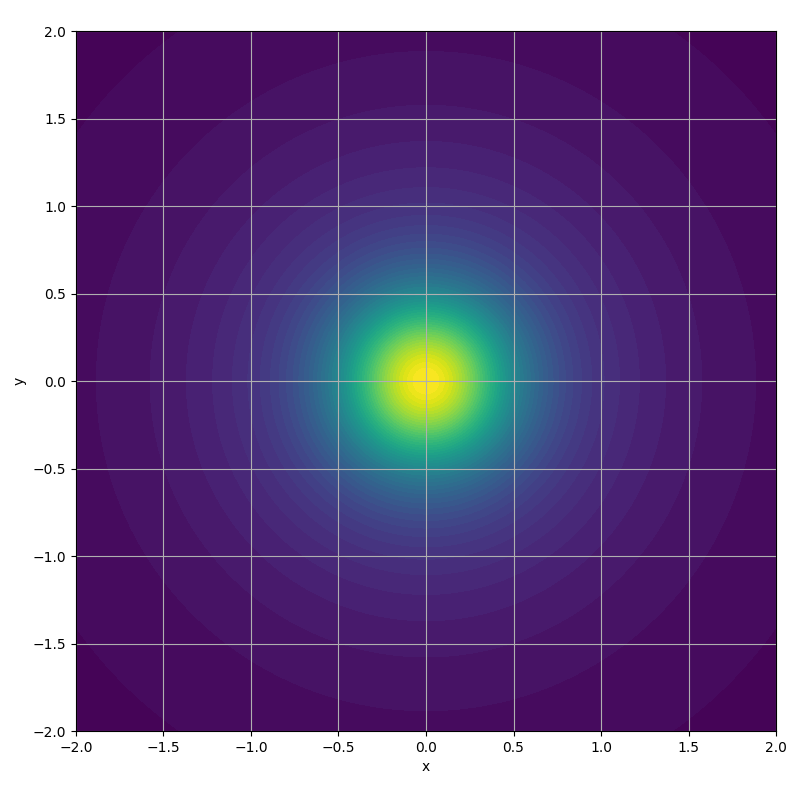
\includegraphics[width=0.5\linewidth]{pictures/Figure_100.png}
\end{figure}

\medskip
\textbf{2. Линейная поляризация: квадрупольный вклад $S_Q$}

Член, пропорциональный $Q$, порождает квадруполь, повернутый на угол $\beta$. При разности распределений 
\[
\dfrac{d\sigma}{d\Omega}(Q) - \dfrac{d\sigma}{d\Omega}(-Q)
\]
изотропная часть исчезает, остаётся чистая квадрупольная картина.

\begin{figure}[H]
\centering
\begin{minipage}{0.45\linewidth}
\centering
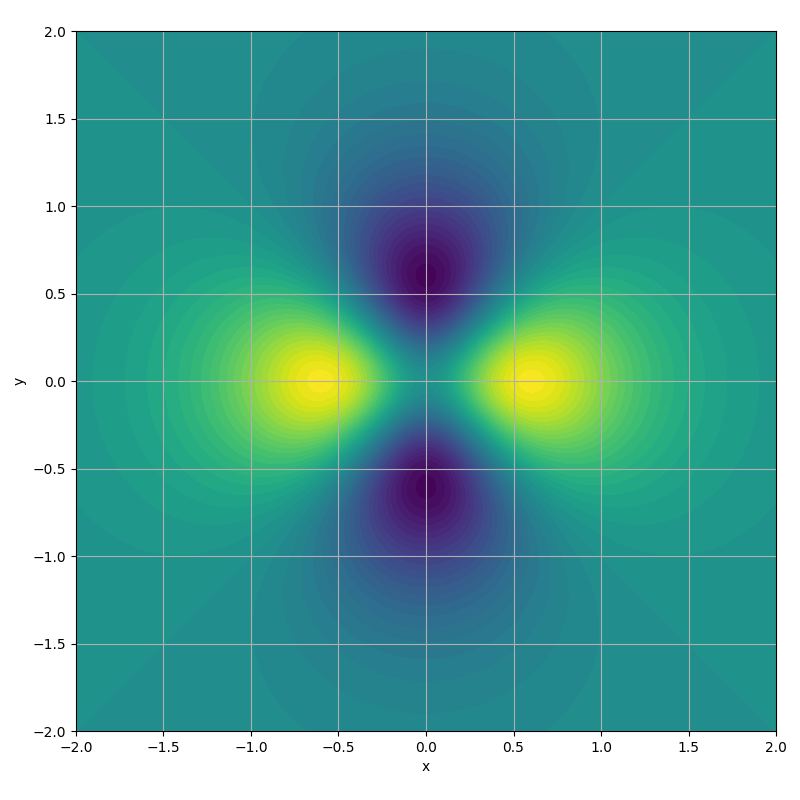
\includegraphics[width=\linewidth]{pictures/квадр 0.png}
\caption{$\beta = 0$}
\end{minipage}
\hfill
\begin{minipage}{0.45\linewidth}
\centering
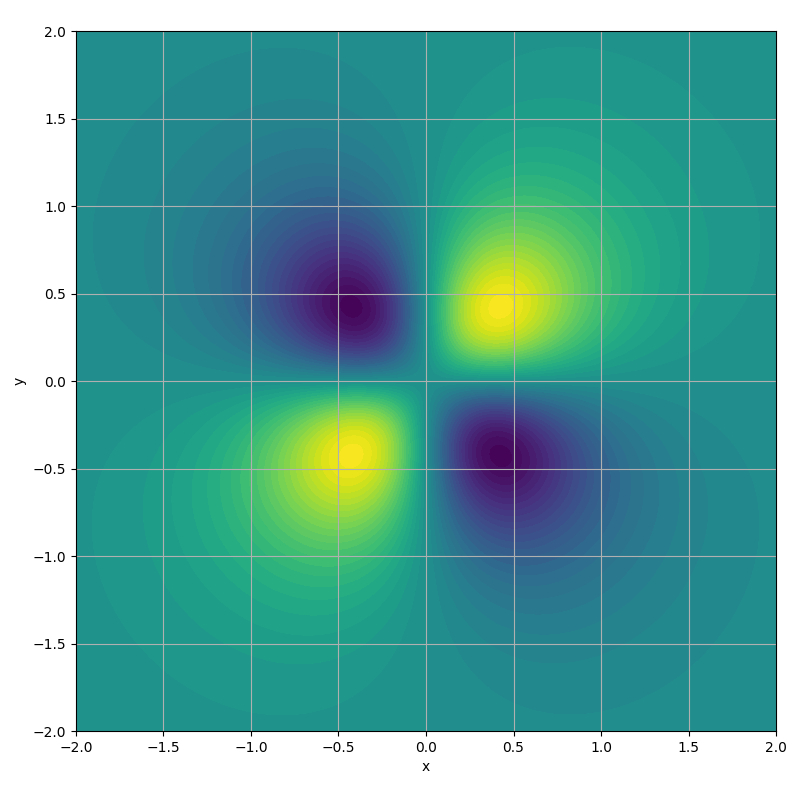
\includegraphics[width=\linewidth]{pictures/квадрi4.png}
\caption{$\beta = \pi/4$}
\end{minipage}
\end{figure}

\begin{figure}[H]
\centering
\begin{minipage}{0.45\linewidth}
\centering
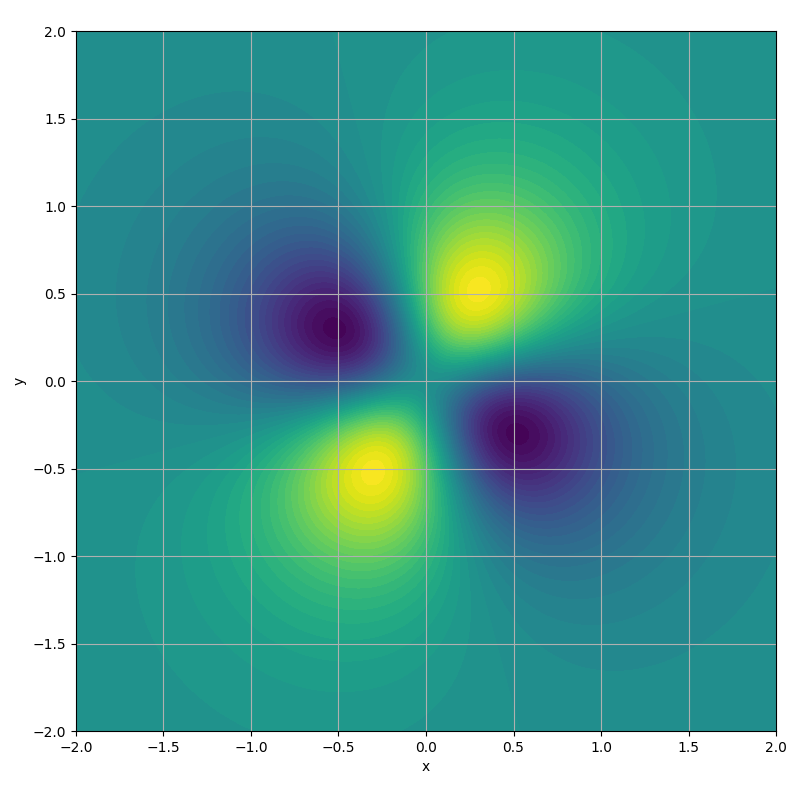
\includegraphics[width=\linewidth]{pictures/квадрпи3.png}
\caption{$\beta = \pi/3$}
\end{minipage}
\hfill
\begin{minipage}{0.45\linewidth}
\centering
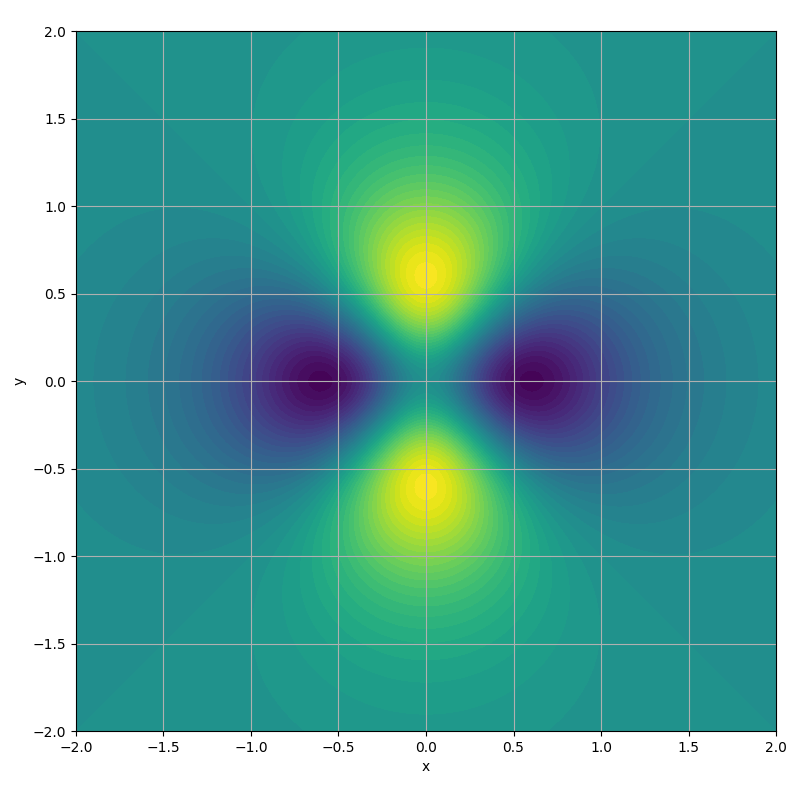
\includegraphics[width=\linewidth]{pictures/квадрпи2.png}
\caption{$\beta = \pi/2$}
\end{minipage}
\end{figure}

\medskip
\textbf{3. Круговая поляризация: дипольный вклад $S_{PV}$}

Член $S_{PV}$ даёт дипольную структуру. Она проявляется только при $PV \neq 0$ и формирует вертикальную асимметрию.

\begin{figure}[H]
    \centering
    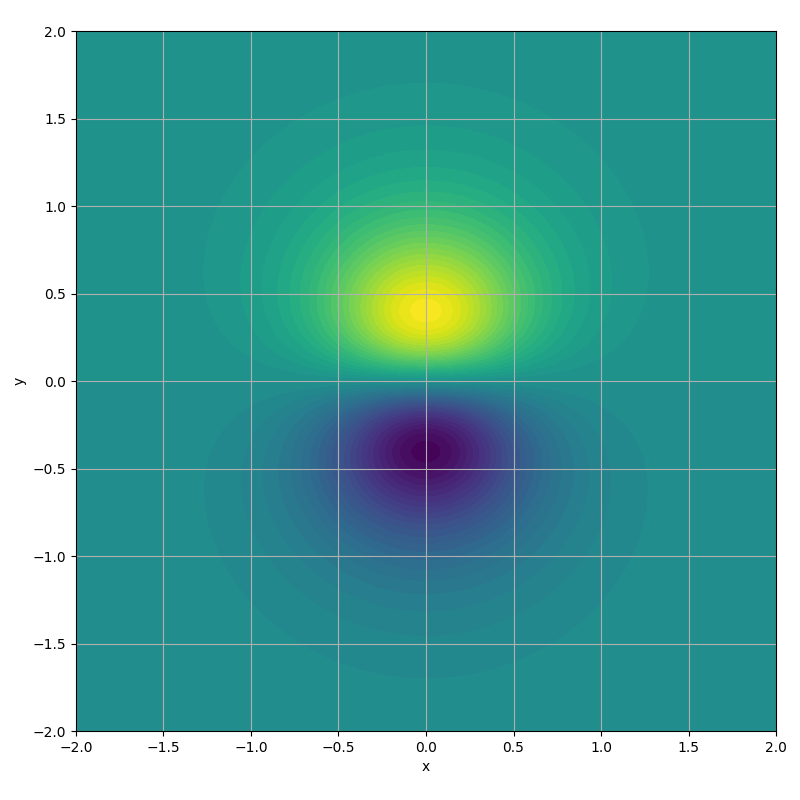
\includegraphics[width=0.45\linewidth]{pictures/дип.png}
\end{figure}

\medskip
\textbf{4. Пример комбинированного вклада}

Пусть $P = 0.6$, $Q = 0.5$, $\beta = \pi/6$.  

Суммарная форма пятна --- результат наложения изотропного фона, квадруполя и диполя.

\begin{figure}[H]
    \centering
    \begin{minipage}{0.22\linewidth}
        \centering
        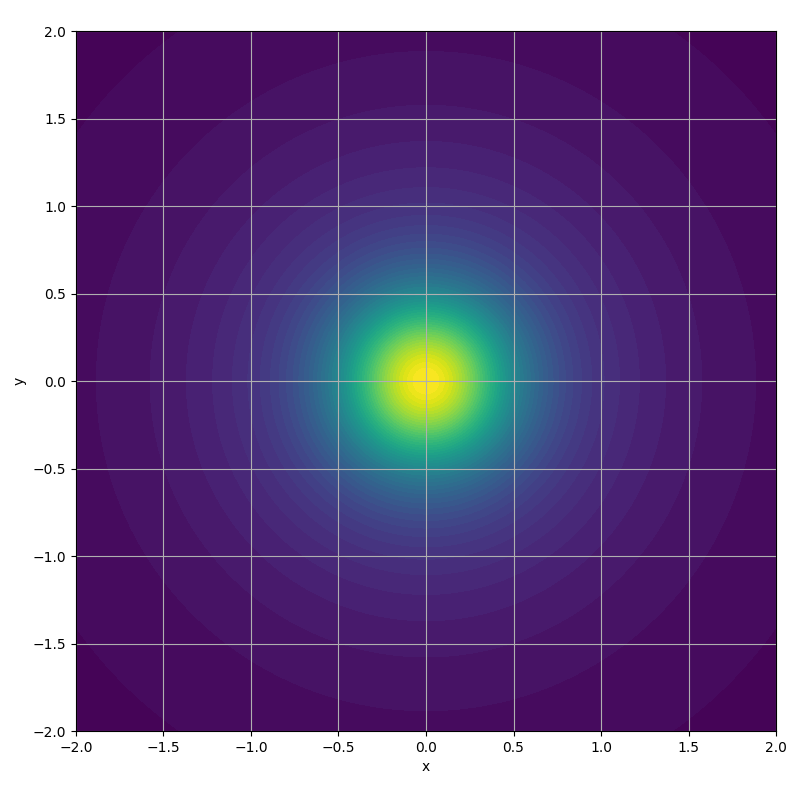
\includegraphics[width=\linewidth]{pictures/nw1.png}
    \end{minipage}
    \hfill
    \Large{$+$}
    \hfill
    \begin{minipage}{0.22\linewidth}
        \centering
        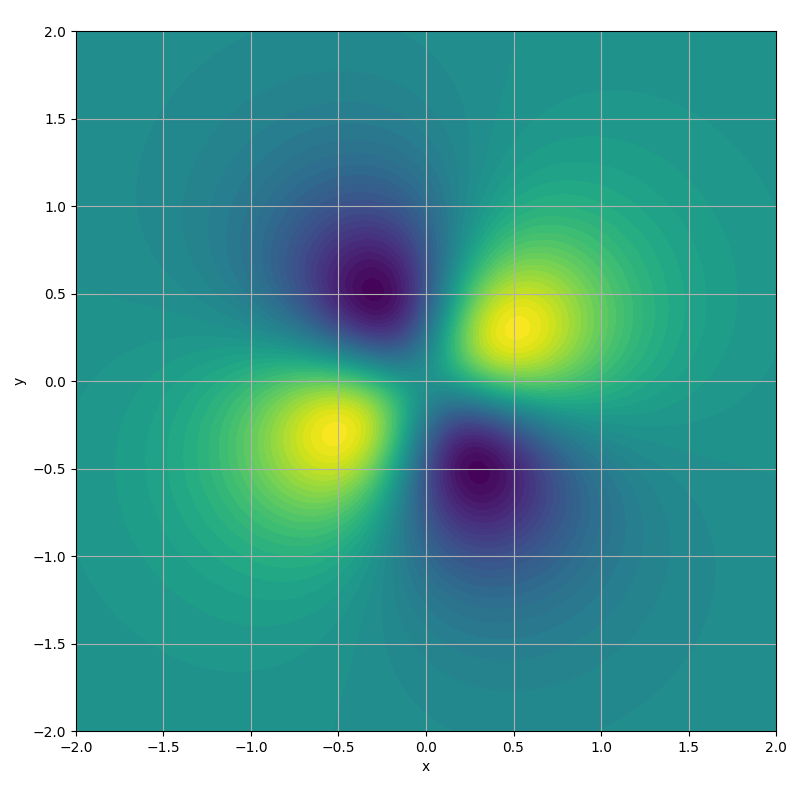
\includegraphics[width=\linewidth]{pictures/new2.png}
    \end{minipage}
    \hfill
    \Large{$+$}
    \hfill
    \begin{minipage}{0.22\linewidth}
        \centering
        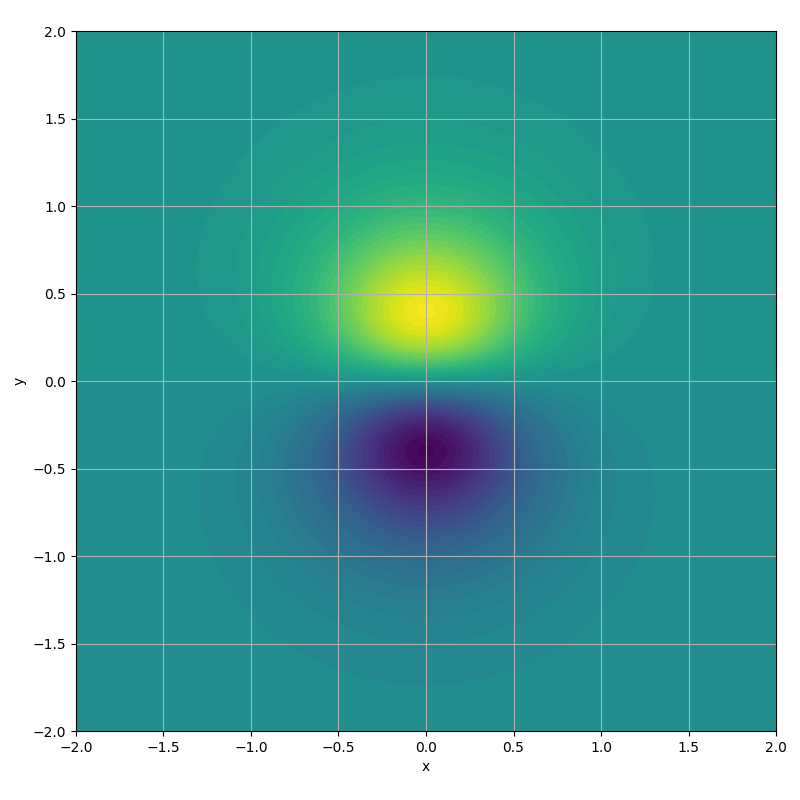
\includegraphics[width=\linewidth]{pictures/nw3.png}
    \end{minipage}
    \hfill
    \Large{$=$}
    \hfill
    \begin{minipage}{0.22\linewidth}
        \centering
        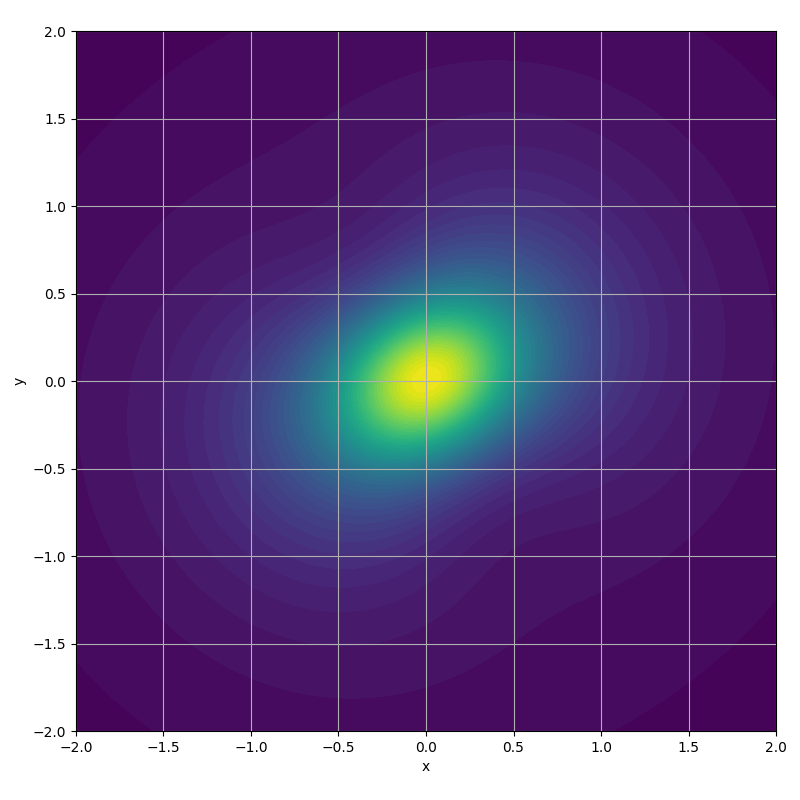
\includegraphics[width=\linewidth]{pictures/dfsdfdjfpiz.png}
    \end{minipage}
\end{figure}

\subsection{Моделирование углов рассеяния}
\subsubsection{Оптимизированный метод Неймана}
Дифференциальное сечение комптоновского рассеяния описывается формулой:
\begin{equation}
\label{eq:cross_section}
\begin{aligned}
\frac{d\sigma}{d\Omega}(\eta, \varphi) &= 2\gamma^{2}r_{e}^{2}
\left[\frac{1}{1+\eta^{2}+\kappa}\right]^{2} \times{} \\
&\quad \times \left(2 + \frac{\kappa^{2}}{(1+\eta^{2})(1+\eta^{2}+\kappa)} 
- \frac{4\eta^{2}}{(1+\eta^2)^{2}}\bigl(1-Q\cos (2[\varphi-\beta])\bigr)\right) + \\
&\quad + 4\gamma^{2}r_{e}^{2}\, PV\, \kappa \frac{\eta\sin\varphi}{(1+\eta^{2})(1+\eta^{2}+\kappa)^{3}}.
\end{aligned}
\end{equation}


Запишем функцию распределения с точностью до константы:
\begin{equation}
\label{eq:density_function}
\begin{aligned}
f(\eta, \varphi) = \frac{C}{\left(1 + \eta^2 + \kappa\right)^2} \Biggl(1 
&+ \frac{\frac{1}{2} \kappa^2}{(1+\eta^2)(1+\eta^2+\kappa)} \\
&- \frac{2\eta^2}{(1+\eta^2)^2}\bigl(1-Q\cos (2[\varphi-\beta])\bigr) \\
&+ \kappa\, PV\, \frac{\eta \sin \varphi}{(1+\eta^2)(1+\eta^2+\kappa)} \Biggr).
\end{aligned}
\end{equation}


Прямое применение метода Неймана к $f(\eta,\varphi)$ неэффективно при больших $\eta$, 
так как плотность по полярному углу быстро убывает как $\sim 1/\eta^3$, и большинство попыток отвергается.

Чтобы ускорить генерацию, выделим из $f(\eta,\varphi)$ множитель, который точно 
интегрируется и хорошо аппроксимирует поведение плотности в хвостах. 
Можно записать в следующей форме:
\begin{equation}
dF = f(\eta, \varphi)\,\eta\, d\eta\, d\varphi = C\,\frac{\eta\, d\eta\, d\varphi}{(1+\eta^2+\kappa)^2}\, B(\eta, \varphi),
\end{equation}
где
\begin{equation}
B(\eta,\varphi) = 1 + \frac{\frac{1}{2}\kappa^2}{(1+\eta^2)(1+\eta^2+\kappa)} 
- \frac{2\eta^2}{(1+\eta^2)^2}\bigl(1-Q\cos(2[\varphi-\beta])\bigr) 
+ \kappa\, PV\, \frac{\eta\sin\varphi}{(1+\eta^2)(1+\eta^2+\kappa)}.
\end{equation}
При больших значениях угла вклад $B(\eta, \varphi)$ ничтожен.

Делаем замену $f(\eta, \varphi)\eta\, d\eta = dG$:
\begin{equation}
dF = B(\eta, \varphi)\, dG\, d\varphi.
\end{equation}

Интегрируя $dG$, получаем:
\begin{equation}
G(\eta) = \int_0^\eta C\,\frac{\eta' d\eta'}{(1+\eta'^2+\kappa)^2} 
= \frac{C\eta^2}{2(1+\kappa)(1+\eta^2+\kappa)}.
\end{equation}

Нормировка:
\begin{equation}
\lim_{\eta \to \infty} G(\eta) = \lim_{\eta \to \infty} 
\frac{C}{2(1+\kappa)\left(1 + \frac{1+\kappa}{\eta^2}\right)} 
= \frac{C}{2(1+\kappa)} = 1 \quad\Rightarrow\quad C = 2(1+\kappa).
\end{equation}

Таким образом,
\begin{equation}
G(\eta) = \frac{\eta^2}{1 + \eta^2 + \kappa}.
\end{equation}

Слишком большие углы можно не учитывать. Выберем $\eta_{\text{max}}$ так, чтобы оно было больше углового разброса в электронном пучке (около $6/\gamma$). Возьмём $\eta_{\text{max}} = 10$.

Случайную величину $\eta$ получаем из условия $G \sim U\!\left(0,\ \dfrac{\eta_{\text{max}}^2}{1+\eta_{\text{max}}^2+\kappa}\right)$:
\begin{equation}
\label{eq: eta}
\eta = \sqrt{\frac{(1+\kappa)G}{1-G}}.
\end{equation}

\textbf{Алгоритм}
\begin{enumerate}
    \item Генерируем случайное число $G \sim U\!\left(0,\ \dfrac{\eta_{\text{max}}^2}{1+\eta_{\text{max}}^2+\kappa}\right)$
    \item Находим $\eta$ по формуле \eqref{eq: eta}.
    \item Выбираем угол $\varphi$ равномерно на $[0, 2\pi)$.
    \item Вычисляем значение скобки $B(\eta,\varphi)$.
    \item Принимаем пару $(\eta,\varphi)$, если случайная величина 
          $u \in [0, B_{\text{max}}]$ удовлетворяет условию $u \le B(\eta,\varphi)$ 
          (метод Неймана). Иначе повторяем сначала.
\end{enumerate}


\subsubsection{Проверка моделирования}


Для проверки подгоним параметры распределения, используя смоделированные этим алгоритмом углы. Для этого подойдет метод максимального правдоподобия.

Разобьем пространство углов на $N$ ячеек. Количество событий в каждой ячейке подчиняется распределению Пуассона.

Вероятность $n_i$ событий в $i$-й ячейке равна:
\begin{equation}
P_i(n_i) = \dfrac{\mu_i^{n_i}e^{-\mu_i}}{n_i!}
\end{equation}

Функция правдоподобия:
\begin{equation}
\ln L\left(P,Q,\beta \right) = \sum_{i=1}^N \left[-\mu_i + n_i \ln(\mu_i) - \ln(n_i!) \right].
\end{equation}
Найдя максимум этой функции, возможно оценить параметры распределения $P^*, Q^*, \beta^*$.

Количество событий -- $10^6$

Гистограммы:

\begin{figure}[H]
    \centering
    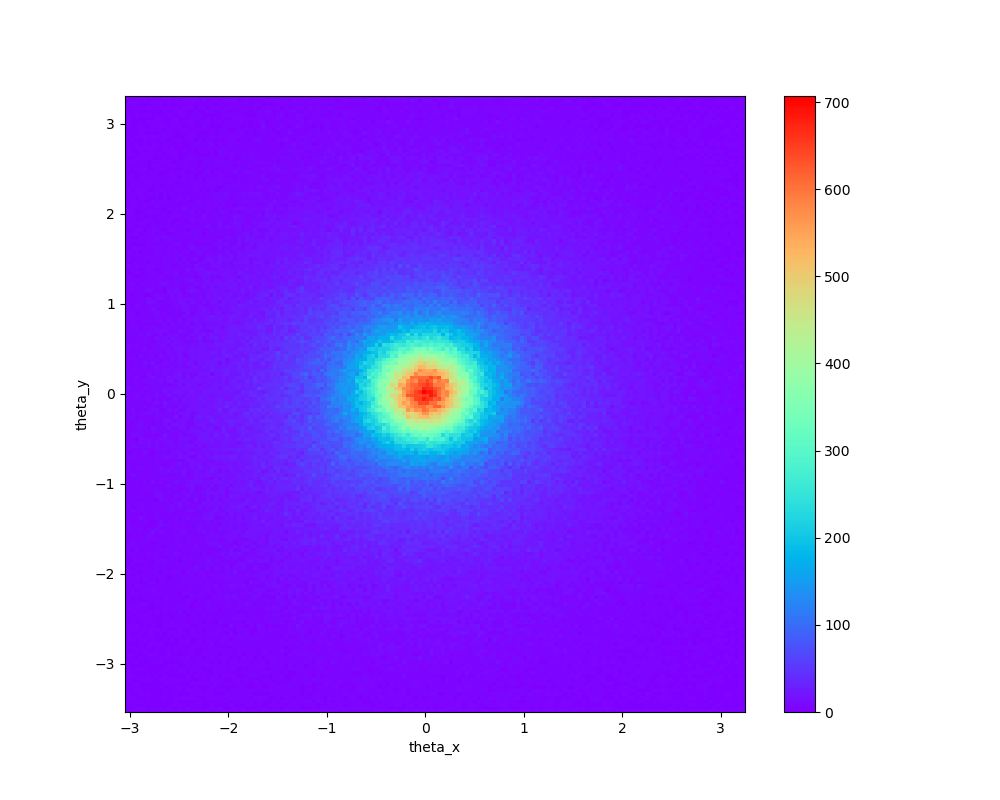
\includegraphics[width=0.7\linewidth]{pictures/Fig_1_0_0.png}
    \caption{$P=1; Q=0; \beta=0.$}
    \label{fig:placeholder}
\end{figure}

\begin{figure}[H]
    \centering
    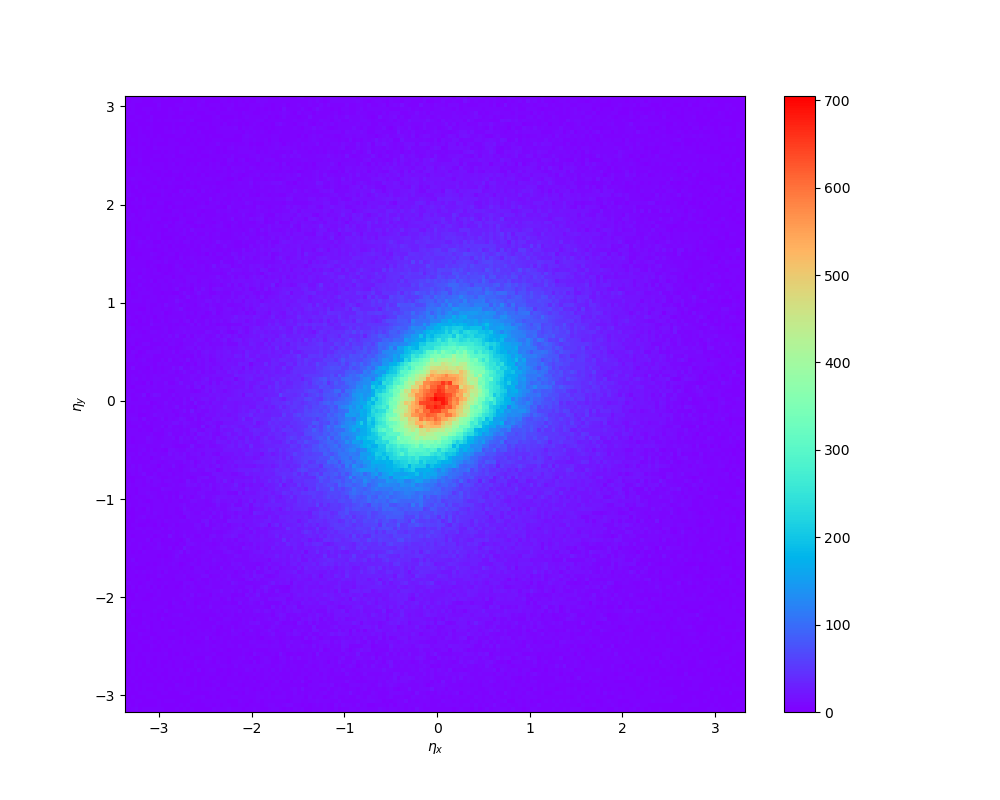
\includegraphics[width=0.7\linewidth]{pictures/Fig_1_0-5_0-7.png}
    \caption{$P=1; Q=0,5; \beta=0,7.$}
    \label{fig:placeholder}
\end{figure}

\begin{figure}[H]
    \centering
    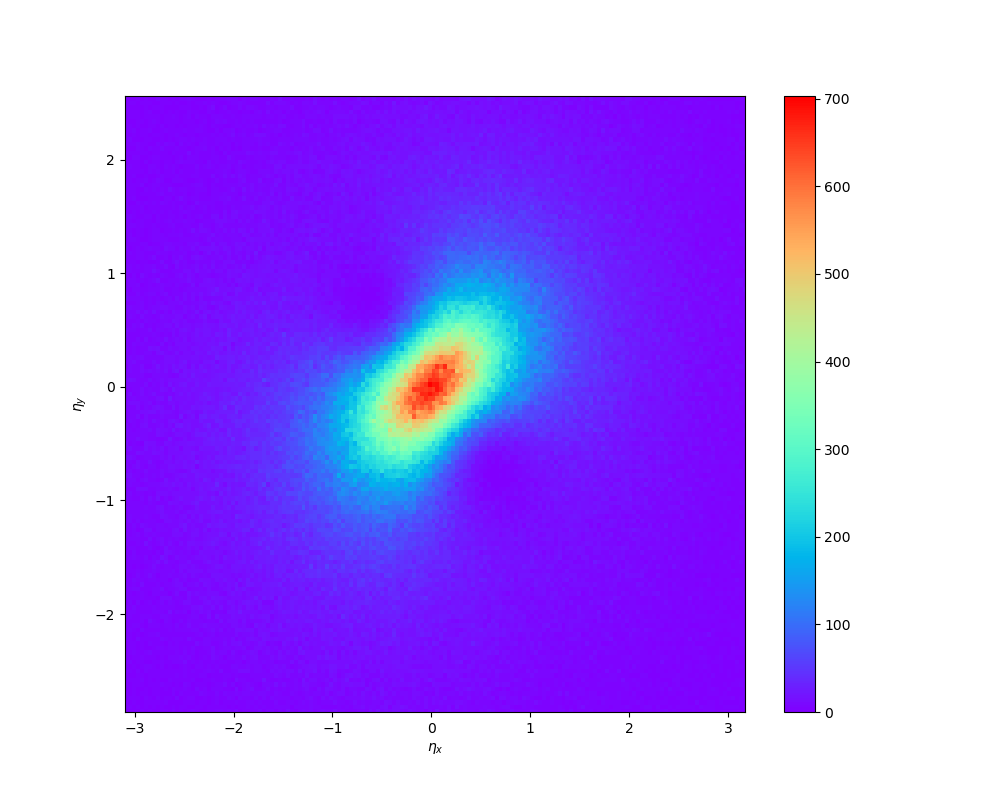
\includegraphics[width=0.75\linewidth]{pictures/figg.png}
    \caption{$P=1; Q=1; \beta=0,7.$}
    \label{fig:placeholder}
\end{figure}

\begin{table}[H]
\centering
\caption{Результаты восстановления параметров}
\begin{tabular}{lccc}
\toprule
Параметр & Истинное значение & Восстановленное значение & Отклонение \\
\midrule
$P$ & 1 & $1,00 \pm 0,06 $& $0$\\
$Q$ & 0 & $0,0042 \pm 0,0024$ & $1,75 \sigma$ \\
$\beta$ (рад) & 0 & $0,85 \pm 0,28$ & $3 \sigma$ \\
\bottomrule
$P$ & 1 & $ 1,00 \pm 0,01 $&  0\\
$Q$ & 0,5 & $ 0,4992 \pm 0,0022$ &  $0,36 \sigma$\\
$\beta$ (рад) & 0,7 & $ 0,6979 \pm 0,0023 $ & $0,91 \sigma$ \\
\bottomrule
$P$ & 1 & $ 0,34 \pm 0,22 $&  $3\sigma$\\
$Q$ & 1 & $ 0,9972 \pm 0,0012$ &  $2,3 \sigma$\\
$\beta$ (рад) & 0,7 & $ 0,6998 \pm 0,0010 $ & $0,2 \sigma$ \\
\bottomrule
\end{tabular}
\end{table}

Графики (синий -- моделирование, красный -- подгонка):
\begin{figure}[H]
    \centering
    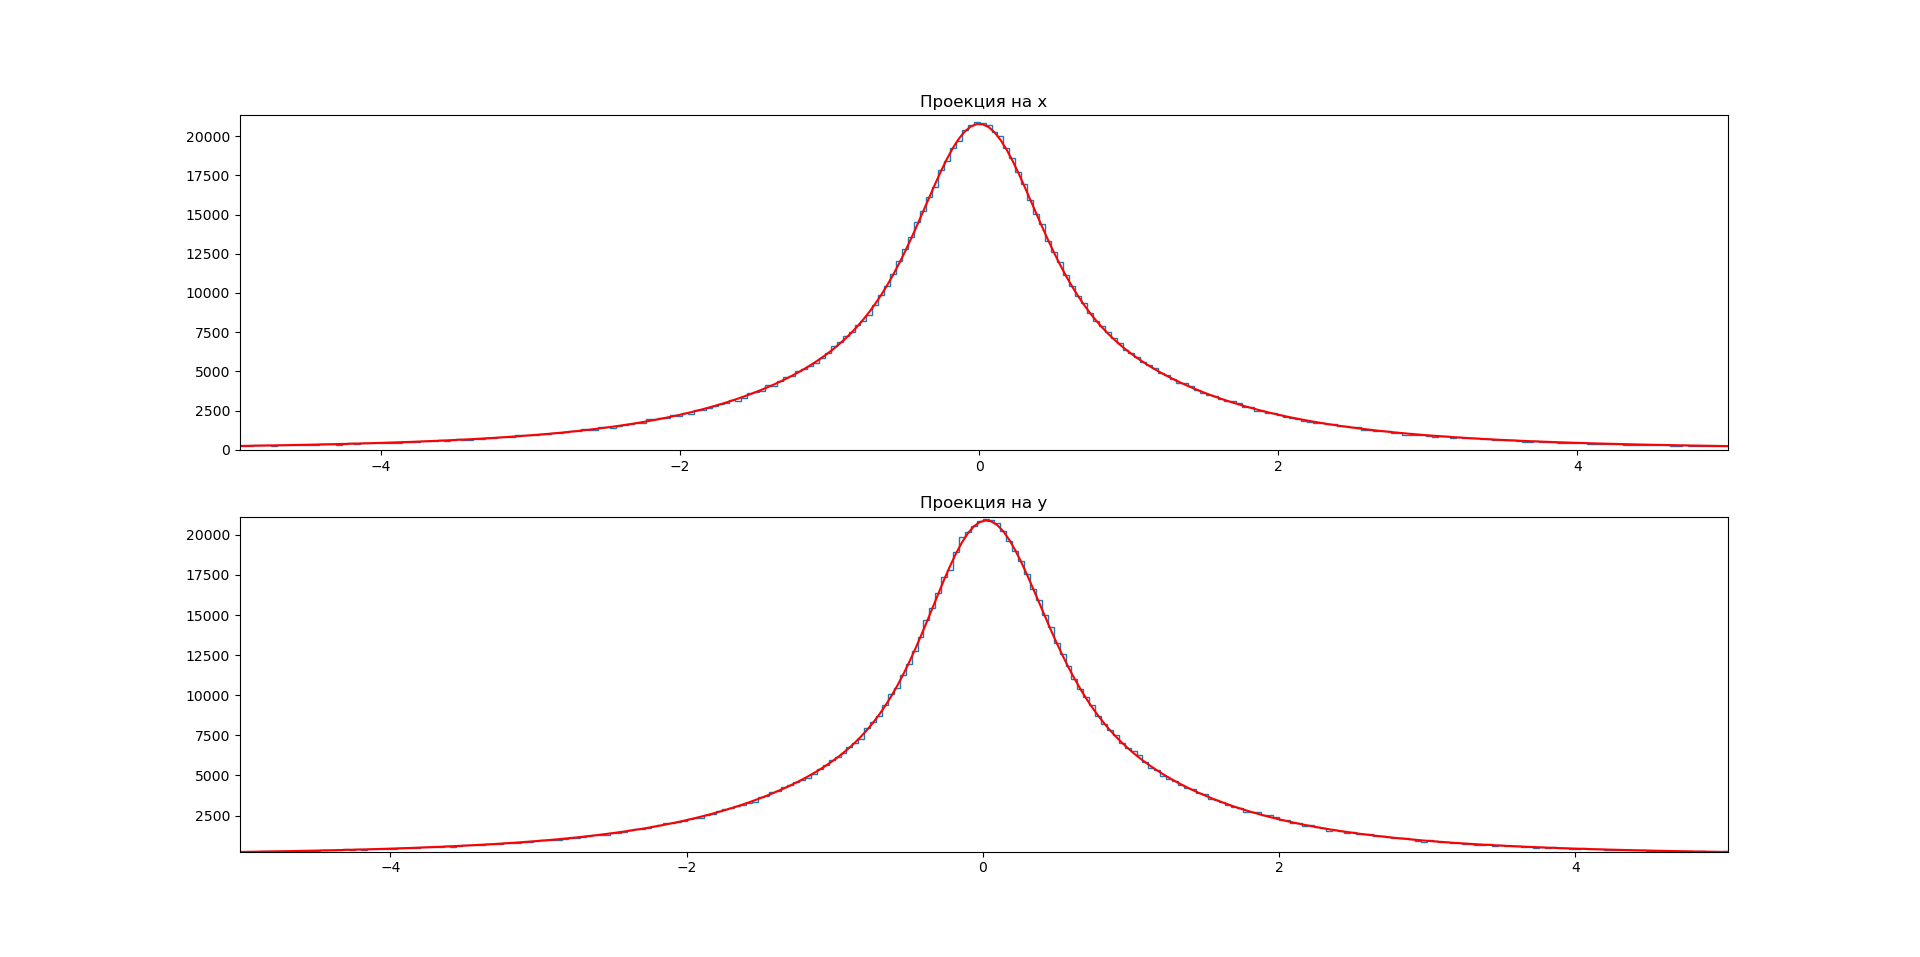
\includegraphics[width=1.\linewidth]{pictures/fit_1_0_0.png}
    \caption{$P=1; Q=0; \beta=0.$}
    \label{fig:placeholder}
\end{figure}

\begin{figure}[H]
    \centering
    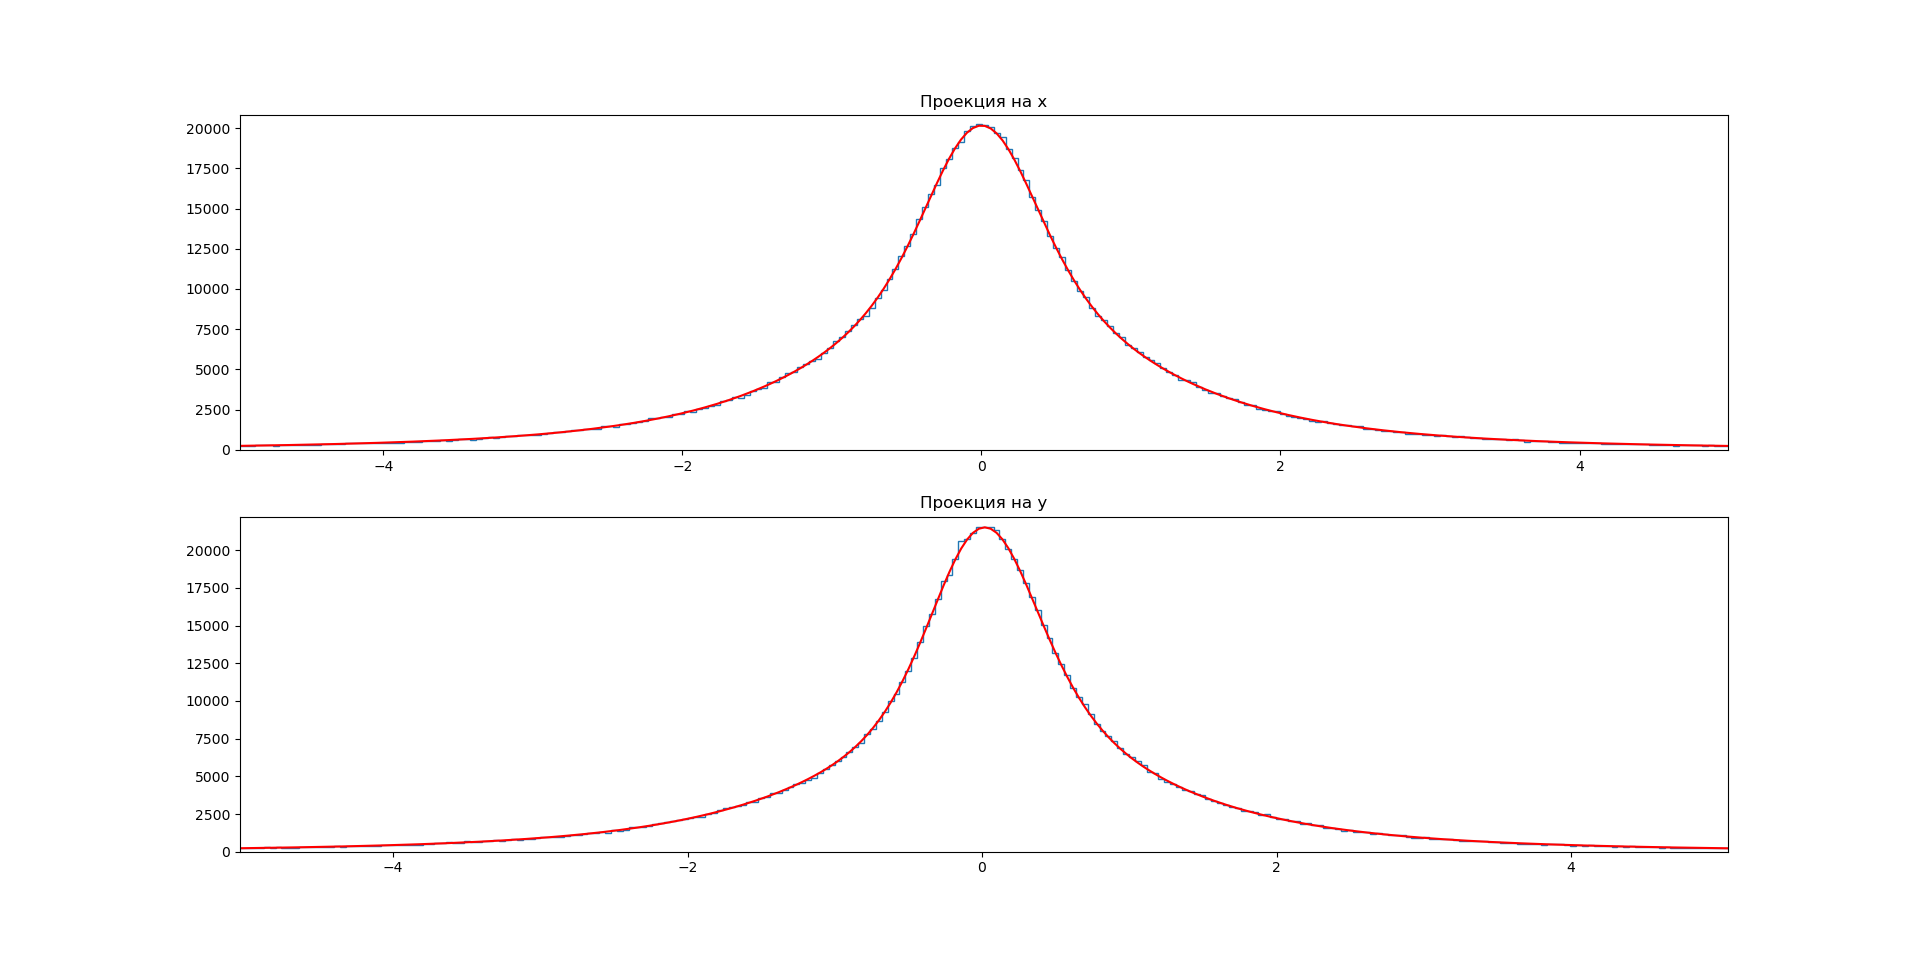
\includegraphics[width=1.\linewidth]{pictures/fit_1_0-5_0-7.png}
    \caption{$P=1; Q=0,5; \beta=0,7.$}
    \label{fig:placeholder}
\end{figure}

\begin{figure}[H]
    \centering
    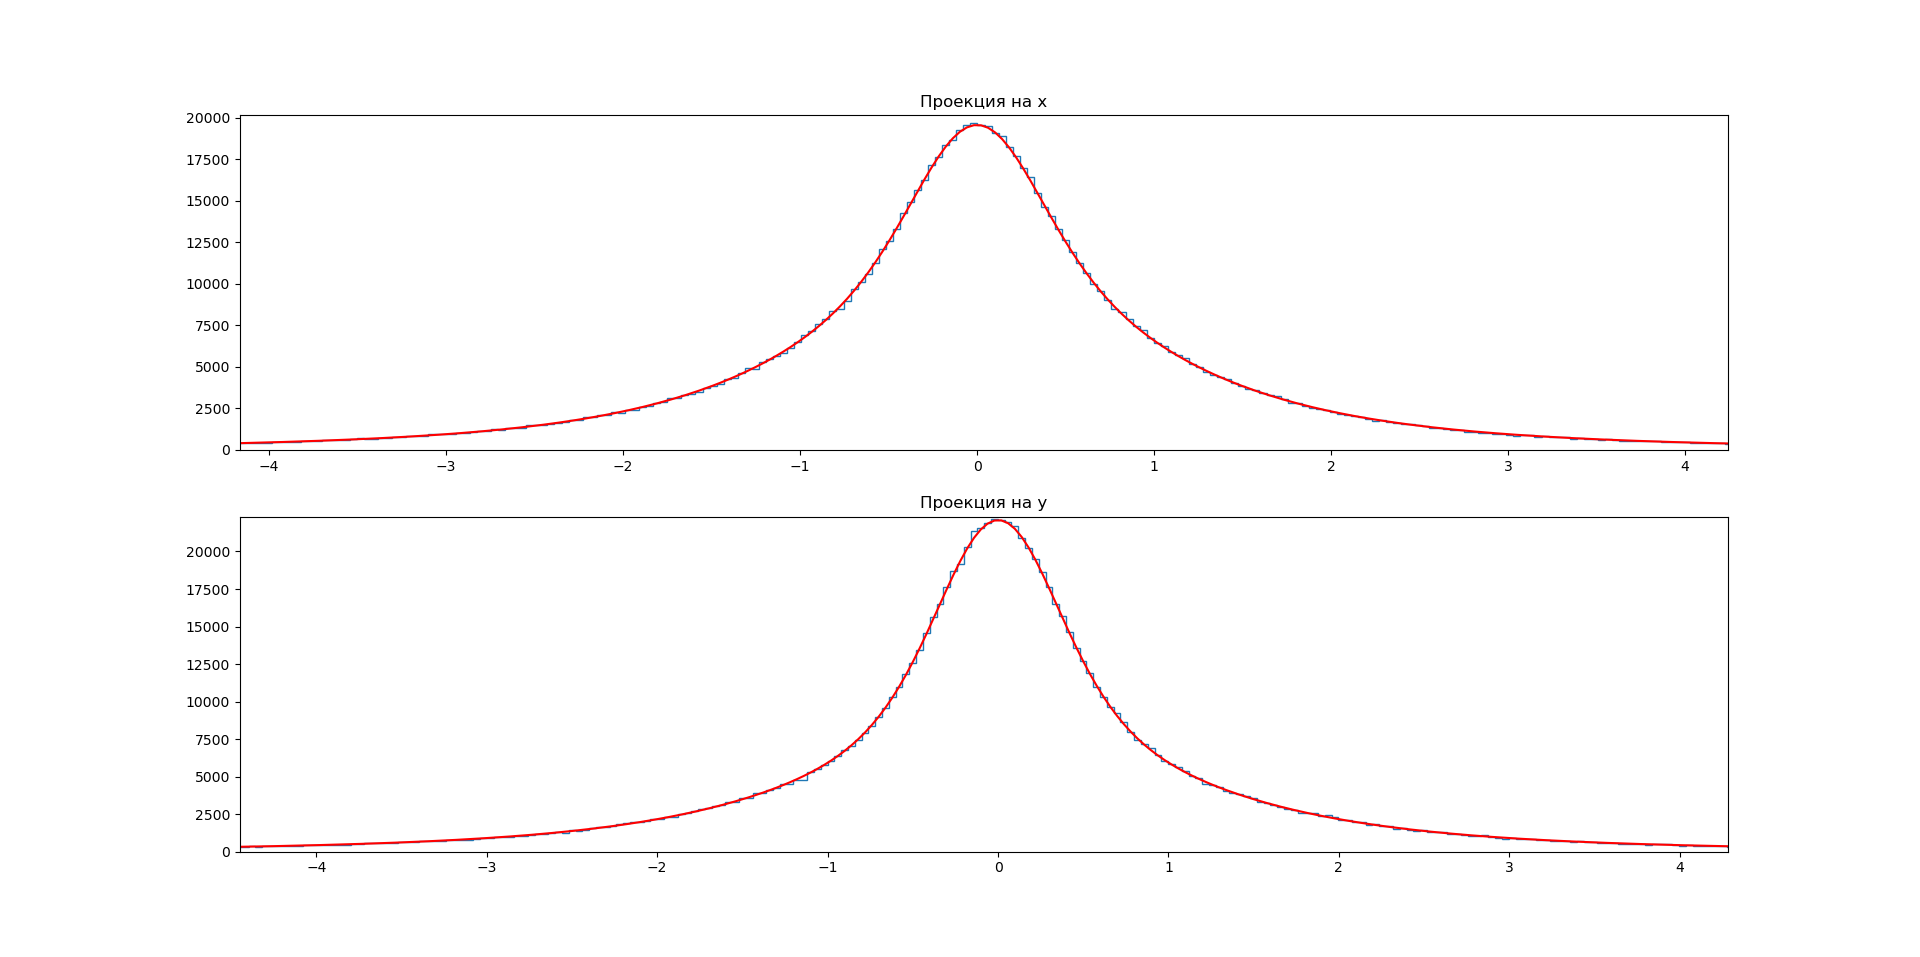
\includegraphics[width=1.\linewidth]{pictures/fittt.png}
    \caption{$P=1; Q=1; \beta=0,7.$}
    \label{fig:placeholder}
\end{figure}

\subsubsection{Анализ результатов}

\textbf{Тест 1} ($Q=0$): Параметр $P$ восстанавливается корректно. Параметр $Q$ восстанавливается относительно хорошо. Угол $\beta$ не может быть определён при $Q=0$, так как квадрупольный член исчезает.

\textbf{Тест 2} ($P=1, Q=0.5$): Все параметры восстанавливаются с высокой точностью. Отклонения не превышают $0.4\sigma$. Это подтверждает корректность работы генератора и процедуры фита в невырожденном случае.

\textbf{Тест 3} ($Q=1, V=0$): Здесь $V = \sqrt{1-Q^2} = 0$. Следовательно, дипольный член $S_{PV}$ исчезает, и поляризация электронов $P$ не может быть определена из данных. Это проявляется в большой погрешности $\pm 0.22$ и смещении оценки $P^* = 0.34 \pm 0.22$. При этом параметры линейной поляризации ($Q$ и $\beta$) восстанавливаются корректно.

\subsection{Рассеяние на электронном пучке}

Ось Z направим против движения первичного фотона. Обозначим $\vartheta - $ угол отклонения направления электрона от оси Z, $\theta - $ угол рассеяния фотона на электроне. Электроны релятивистские, значит, углы малы и мы можем рассматривать угловые отклонения от оси как векторы на касательной к сфере плоскости в точке её пересечения с этой осью. Базис -- декартовы орты.

\begin{equation}
    \bm{\theta}_e = (\vartheta \cos \phi, \vartheta \sin \phi)
\end{equation}

\begin{equation}
    \bm{\theta}_{\gamma} = (  \theta \cos \varphi ,\theta \sin \varphi)
\end{equation}
Для вектора отклонения фотона имеем
\begin{equation}
    \label{eq:delta}
    \bm{\delta} =  \bm{\tau}_{\gamma} + \bm{\tau}_e = (\vartheta \cos \phi +  \theta \cos \varphi, \vartheta \sin \phi +  \theta \sin \varphi ) 
\end{equation}

А его длина равна
\begin{equation}
    \delta^2 = (\vartheta \cos \phi +  \theta \cos \varphi)^2 + (\vartheta \sin \phi +  \theta \sin \varphi)^2
\end{equation}



Формула \eqref{eq:compt_en} для энергии рассеянного фотона через углы $\theta, \vartheta,\delta$:
\begin{equation}
    \label{eq:energy}
     \omega' = \omega \dfrac{1 + \beta\cos\vartheta }{1 - \beta \cos\theta + \dfrac{\omega}{\varepsilon}\left(1+\cos \delta\right)}
\end{equation}
\textbf{Дополнение к алгоритму}
\begin{enumerate}
    \item Генерируем координаты электрона по гауссу.
    \item Генерируем разброс электрона по гауссу.
    \item Складываем углы разброса с углами, сгенерированными по алгоритму, согласно \eqref{eq:delta}.
    \item Вычисляем энергию по формуле \eqref{eq:energy}.
    \item Запускаем фотон с заданными координатами, углами и энергией.
\end{enumerate}
\newpage
\section{Физика взаимодействия излучения с веществом}
В данном разделе кратко рассматриваются физические процессы, существенные для описываемого эксперимента.

\subsection{Фотоэффект}
Фотоэффектом называется явление выбивания фотоном электрона из атома:
\begin{equation}
    \gamma + e^* \rightarrow e,
\end{equation}
где $e^*$ — связанный электрон.

\paragraph{Сечение фотоэффекта}
Фотоэффект возможен только на связанном электроне, причём вероятность взаимодействия тем выше, чем сильнее эта связь. Процесс преимущественно идёт с участием электронов $K$-оболочки, обладающих наибольшей энергией связи в атоме. Сечение на весь атом составляет:
\begin{equation}
    \sigma_{\text{атом}} \approx \frac{5}{4}\sigma_K.
\end{equation}

\begin{figure}[H]
    \centering
    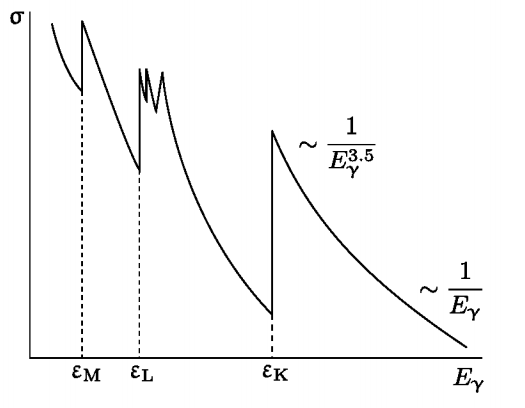
\includegraphics[width=0.5\linewidth]{pictures/сечение фотоэффекта.png}
    \caption{Зависимость сечения фотоэффекта от энергии фотона}
    \label{fig:photor}
\end{figure}

Для $K$-оболочки справедливы следующие приближения:
\begin{itemize}
    \item При $\varepsilon_K \ll E_{\gamma} \ll mc^2$:
    \begin{equation}
        \sigma_K = 10^{-33} \frac{Z^5}{E_{\gamma[\text{МэВ}]}^{3,5}}\ \text{см}^2.
    \end{equation}
    \item При $E_{\gamma} \gg mc^2$:
    \begin{equation}
        \sigma_K = 1,4 \cdot 10^{-33} \frac{Z^5}{E_{\gamma[\text{МэВ}]}}\ \text{см}^2.
    \end{equation}
\end{itemize}

При приближении энергии фотона к энергии связи электрона на $K$-оболочке сечение растёт как $E_{\gamma}^{-3,5}$, а при высоких энергиях — как $E_{\gamma}^{-1}$. Характерной особенностью фотоэффекта является сильная зависимость от атомного номера $Z$ (энергия связи на $K$-оболочке $\sim Z^2$). Поэтому фотоэффект играет ключевую роль для тяжёлых веществ.

\subsection{Эффект Комптона}
Эффект Комптона представляет собой рассеяние фотона на свободном электроне:
\begin{equation}
    \gamma + e \rightarrow \gamma' + e'.
\end{equation}

Полное сечение на покоящемся электроне:
\begin{itemize}
    \item При $E_{\gamma} \ll mc^2$ (томсоновское рассеяние):
    \begin{equation}
        \label{eq:thomson_scattering}
        \sigma = \frac{8}{3}\pi r_0^2.
    \end{equation}
    \item При $E_{\gamma} \gg mc^2$:
    \begin{equation}
        \label{eq:compt_scattering}
        \sigma = \pi r_0^2 \frac{mc^2}{E_{\gamma}} \left[ \ln\left( \frac{2E_{\gamma}}{mc^2} \right) + \frac{1}{2} \right].
    \end{equation}
\end{itemize}

При малых энергиях фотона сечение комптоновского рассеяния не зависит от энергии и определяется томсоновским сечением; с ростом энергии оно уменьшается.

\subsection{Рождение пар}
Рождение пар — это процесс образования электрон-позитронной пары фотоном в поле ядра:
\begin{equation}
    \gamma + Z \rightarrow e^+ + e^- + Z.
\end{equation}

В данном случае удобнее использовать коэффициент поглощения. Начиная от порога реакции, коэффициент поглощения логарифмически растёт с увеличением энергии и при больших энергиях асимптотически выходит на постоянный уровень.

\begin{figure}[H]
    \centering
    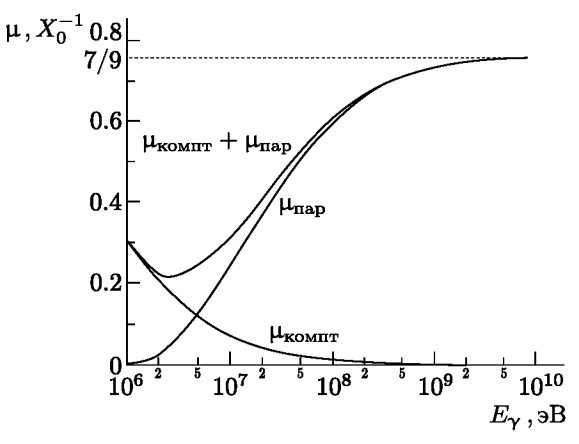
\includegraphics[width=0.5\linewidth]{par.png}
    \caption{Коэффициент поглощения фотонов за счёт рождения пар и комптоновского рассеяния}
    \label{fig:placeholder}
\end{figure}

\begin{itemize}
    \item При $m_ec^2 \ll E_{\gamma} \ll 137 m_ec^2 Z^{-1/3}$:
    \begin{equation}
        \mu_{\text{пар}} = \frac{7}{9}\frac{1}{X_0}\frac{\ln\left( \frac{2E_{\gamma}}{mc^2} \right) - 2,6}{\ln\left(183 Z^{-1/3} \right)}.
    \end{equation}
    \item При $E_{\gamma} \gg 137 m_ec^2 Z^{-1/3}$:
    \begin{equation}
        \mu_{\text{пар}} = \frac{7}{9}\frac{1}{X_0}.
    \end{equation}
\end{itemize}

Грубо можно считать, что электроны и позитроны рождаются с равной вероятностью во всём допустимом диапазоне энергий. Однако на практике позитрон, будучи положительно заряженным, как и ядро, несколько чаще обладает большей энергией, чем электрон.


\subsection{Суммарный коэффициент поглощения фотонов}
Полный коэффициент поглощения складывается из вкладов фотоэффекта, комптоновского рассеяния и рождения пар:
\begin{equation}
    \mu = \mu_{\text{фото}} + \mu_{\text{компт}} + \mu_{\text{пар}}.
\end{equation}

Коэффициент поглощения связан с сечением соотношением:
\begin{equation}
    \mu = \frac{N_0}{A} \rho \sigma_{\text{атом}}.
\end{equation}

Важно учитывать, что теория Клейна–Нишины–Тамма даёт сечение комптоновского рассеяния на одном электроне, поэтому при вычислении $\mu_{\text{компт}}$ в веществе выражения \eqref{eq:thomson_scattering} и \eqref{eq:compt_scattering} необходимо умножить на $Z$.

\begin{figure}[H]
    \centering
    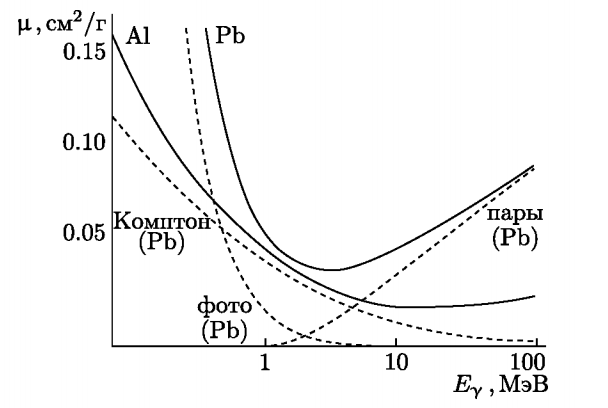
\includegraphics[width=0.5\linewidth]{mu_sum.png}
    \caption{Суммарный коэффициент поглощения фотонов}
    \label{fig:placeholder}
\end{figure}

\subsection{Ионизационные потери}
Электрон или позитрон, пролетая через вещество, может вырвать электрон из атома (ионизация), теряя при этом часть своей энергии. Эти потери называются ионизационными.

Формула для ионизационных потерь электронов:
\begin{equation}
    -\frac{dT}{dx} = \frac{2\pi e^4 n_e}{m_e v^2} \left[ \ln \frac{m_e v^2}{2I^2(1-\beta^2)} - \ln 2\left(2\sqrt{1-\beta^2} - 1 + \beta^2\right) + 1 - \beta^2 + \frac{1}{8}\left(1 - \sqrt{1-\beta^2}\right)^2 - \delta \right],
\end{equation}
где $I \approx 16Z$ эВ — средний потенциал ионизации атомов поглощающего вещества, $\delta$ — поправка на эффект плотности.

\subsection{Тормозное излучение}
При пролёте электрона вблизи ядра его траектория искривляется под действием кулоновской силы, т.е. электрон движется с ускорением $a$ и излучает с мощностью $P = \frac{2}{3}\frac{e^3}{c^3}a^2$. Этот процесс описывается как:
\begin{equation}
    e + Z \rightarrow e + Z + \gamma.
\end{equation}

\begin{itemize}
    \item При $m_ec^2 \ll E_{\gamma} \ll 137 m_ec^2 Z^{-1/3}$:
    \begin{equation}
        -\frac{dE_{\text{изл}}}{dx} = \frac{E}{X_0}\frac{\ln\left( \frac{2E_{\gamma}}{mc^2} \right) - \frac{1}{3}}{\ln\left(183 Z^{-1/3} \right)}.
    \end{equation}
    \item При $E_{\gamma} \gg 137 m_ec^2 Z^{-1/3}$:
    \begin{equation}
        -\frac{dE_{\text{изл}}}{dx} = \frac{E - mc^2}{X_0}\frac{\ln\left(183 Z^{-1/3} \right) + \frac{1}{18}}{\ln\left(183 Z^{-1/3} \right)} \approx \frac{E}{X_0}.
    \end{equation}
\end{itemize}


\subsection{Многократное рассеяние}
Пучок частиц, падая на слой вещества, испытывает не только ионизационные потери, но и многократные рассеяния на ядрах. В результате большого числа столкновений частицы выходят из вещества под некоторым углом $\alpha$ к первоначальному направлению. Этот угол зависит от типа вещества и толщины слоя, а также от типа частиц. Вследствие изотропии вещества углы $+\alpha$ и $-\alpha$ равновероятны, поэтому средний угол рассеяния равен нулю. Более информативной характеристикой является среднеквадратичный угол.

Формула Росси для электронов:
\begin{equation}
    \sqrt{\overline{\theta^2}} = \frac{21\ \text{МэВ}}{p\beta c} \sqrt{\frac{x}{X_0}}.
\end{equation}
\section{Моделирование в Geant4}

В этом разделе будет проделано моделирование прохождения рассеянных жёстких фотонов через экспериментальную установку.
\subsection{Геометрия установки}
Установка включает в себя следующие ключевые элементы:
\begin{itemize}
\item \textbf{Фланец вакуумной трубы}: диаметр --- 40 мм, толщина --- 1,5 мм.
\item \textbf{Зеркало:} диаметр --- 100 мм, толщина медного зеркала --- 4 мм, толщина водного слоя --- 17 мм, толщина стальных стенок (по обе стороны водного слоя) --- 1 мм.
\item \textbf{Конвертер:} материал --- свинец, толщина --- 12 мм), ширина --- 161,4 мм, высота --- 50,35 мм. Расположен на расстоянии 29,9 м от области взаимодействия лазера с пучком.
\item \textbf{Упрощённая модель детектора:} на данном этапе представлена тонким слоем аргона, регистрирующим координаты (x, y) заряженных частиц. Полноценная модель ГЭУ с падами и лавинным умножением будет реализована на следующем этапе.

\end{itemize}
\begin{figure}[H]
\centering
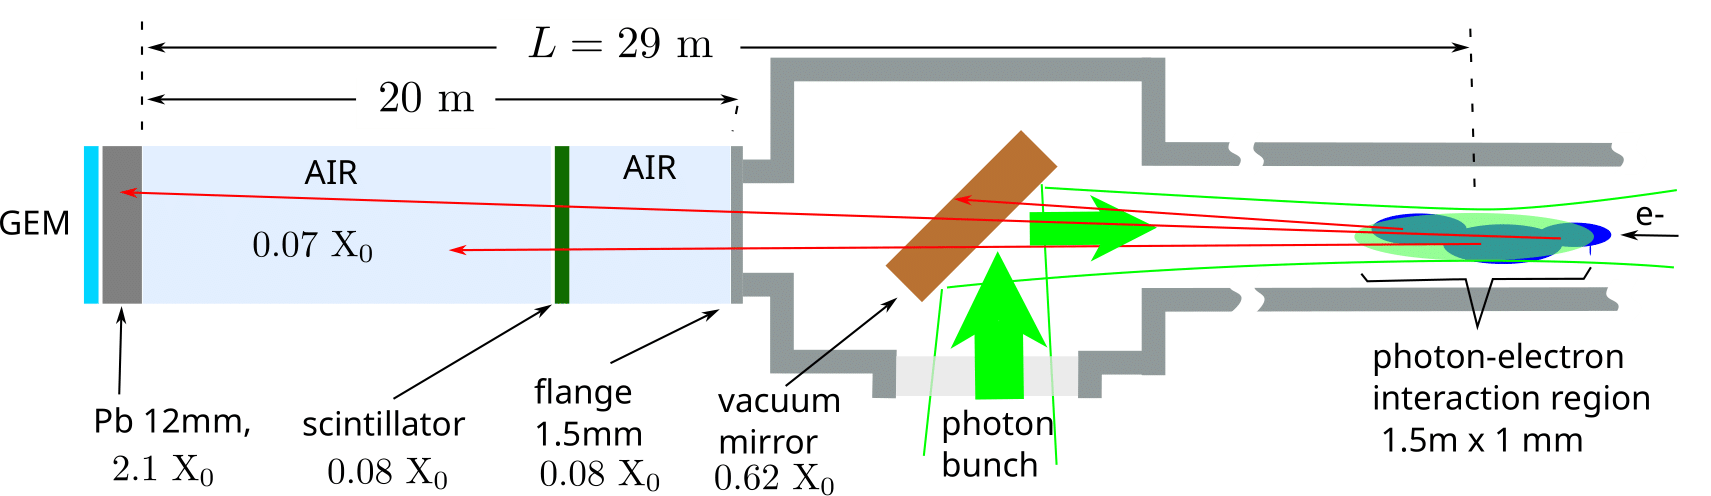
\includegraphics[scale=0.7]{pictures/material_scheme-1.png}
\caption{Схематичное изображение установки.}
\end{figure}

\subsection{Реализация физики}


Для корректной реализации всех электромагнитных процессов, в основном --- ливней в конвертере, в Geant4 выбран список физики для электромагнетизма. Он включает:
\begin{itemize}
\item Для фотонов: фотоэффект, комптоновское рассеяние, рождение пар.
\item Для электронов/позитронов: ионизационные потери, тормозное излучение, множественное рассеяние.
\begin{figure}[H]
\centering
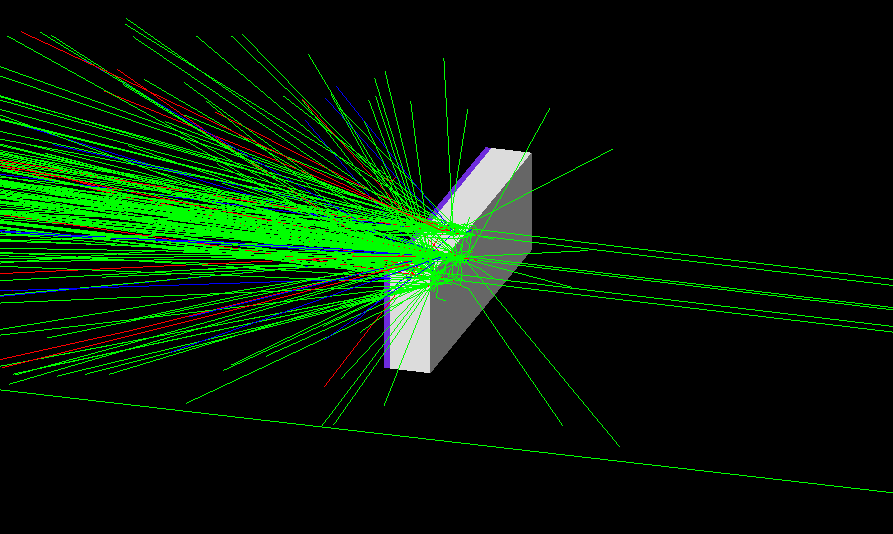
\includegraphics[scale=0.4]{pictures/rain.png}
\caption{Ливень в конвертере.}
\end{figure}
\end{itemize}


\subsection{Конвертер}
Конвертер нужен для превращения фотонов в электрон-позитронные пары, которые проще детектировать. Как мы видим, для энергии фотонов в нашем эксперименте рождение пар преобладает над другими процессами, что оправдывает использование конвертера. Эффективность конвертера тем выше, чем сильнее фотоны взаимодействуют с металлом. Посмотрим как зависит вероятность взаимодействия от толщины для разных металлов. 
\subsubsection{Вероятность взаимодействия фотона с веществом}
Для этого проведём следующее моделирование в Geant4: разместим конвертер заданной толщины и материала на пути к фотонам и будем считать количество провзаимодействовавших с ним. 
Ниже приведена таблица, в которой отражена зависимость числа провзаимодействовавших фотонов от толщины разных металлов.
\\
Количество налетающих фотонов -- 100 000.


\begin{figure}[H]
    \centering
    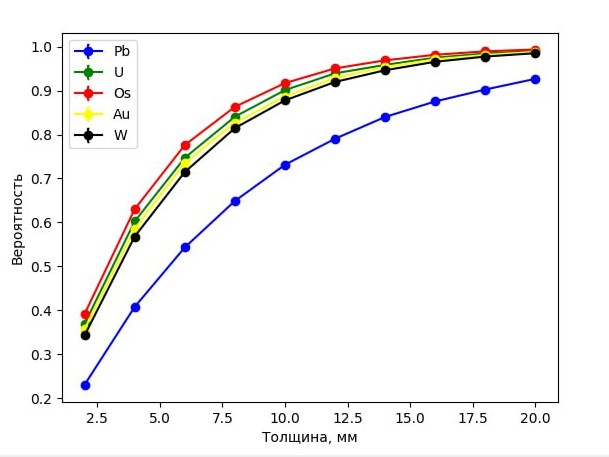
\includegraphics[width=0.7\linewidth]{pictures/fbc984ea-c7c6-41c1-b77b-5bc2c498663d.jpeg}
    \caption{Зависимость вероятности взаимодействия $\gamma-$кванта с энергией 800 МэВ с различными металлами от их толщины. }
    \label{fig:prob}
\end{figure}
\subsubsection{Оптимальная толщина конвертера}
Конвертер служит для преобразования фотонов в электрон-позитронные пары. 
Далее заряженные частицы фиксируются на детекторе, на основе этих данных проводится подгонка изначального распределения фотонов.
В области малых толщин эффективность подгонки быстро растёт, поскольку большее число фотонов участвует в рождении пар, что увеличивает количество регистрируемых событий. Однако при больших толщинах количество взаимодействующих фотонов выходит на плато и начинает доминировать многократное рассеяние электронов и другие электромагнитные процессы, приводящие к уширению пятна и постепенной потере информации о поляризации.

Зависимость эффективности подгонки поляризации 
\[
\frac{P^*}{\sigma_{P^*}}
\]
от толщины конвертера хорошо аппроксимируется гамма-распределением 
\begin{figure}[H]
    \centering
    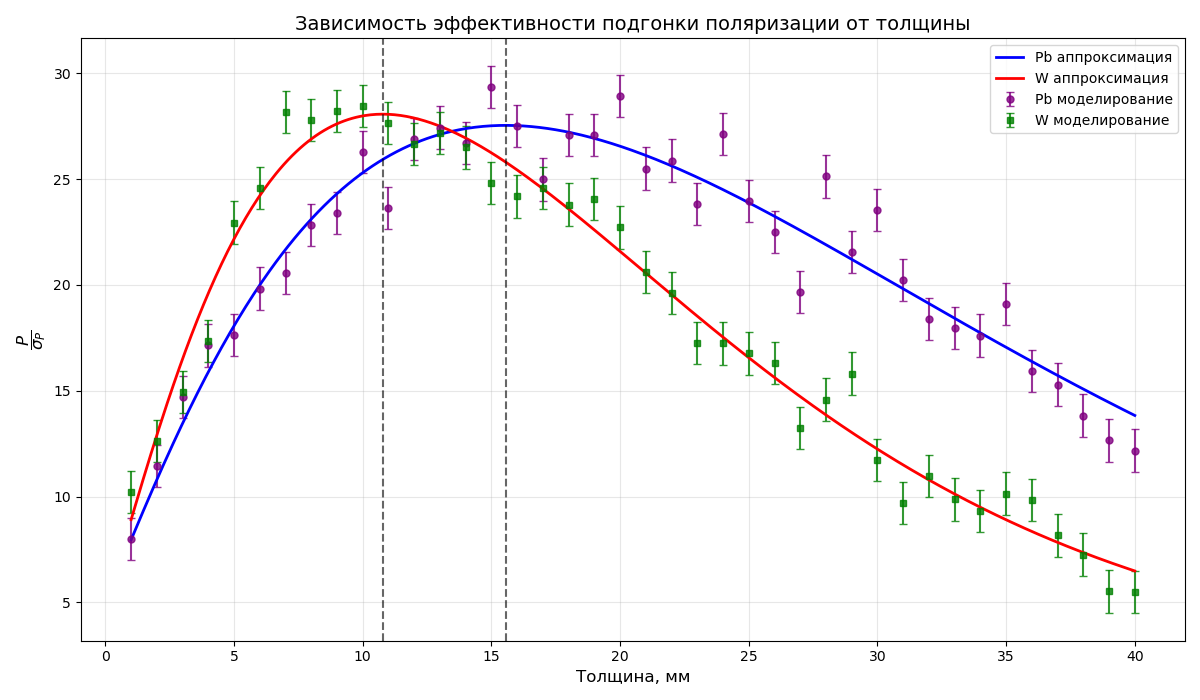
\includegraphics[width=0.7\linewidth]{fitting.png}
    \caption{Зависимость эффективности подгонки поляризации от толщины конвертера из свинца/вольфрама}
    \label{fig:wolphram}
\end{figure}

\begin{table}[h]
\centering
\begin{tabular}{l|c|c|}
\cline{2-3}
                     & $\chi^2/ndf$          & Оптимальная толщина, мм          \\ \hline
\multicolumn{1}{|l|}{Свинец} & 2,272 & 15,56\\ \hline
\multicolumn{1}{|l|}{Вольфрам} & 1,406  & 10,78 \\ \hline
\end{tabular}
\end{table}

По графику видно, что гамма-распределение хорошо подгоняет данные, но $\chi^2$ слишком велик. Это происходит из-за проблем с моделью при подгонке. Возникает систематическая ошибка.

Также из графика видно, что смена свинцового конвертера на вольфрамовый не даёт сильного повышения эффективности, а значит в этом нет нужды. 
\subsection{Детектор}
\subsubsection{Порог заряда на детекторе.}
Сначала построим гистограмму заряда на падах.
\section{Обработка данных}

Данные на детекторе
\begin{equation}
    D^{L,R}(x,y) = \int B(x,y,\theta_x, \theta_y)C^{L,R}(\theta_x,\theta_y)d\theta_xd\theta_y \approx \dfrac{1}{L^2}\int B(x-x', y-y')C^{L,R}\left(\dfrac{x'}{L}, \dfrac{y'}{L}\right)dx'dy'
    \end{equation}
Нужно найти $B(x,y)$.

Пользуясь свойством Фурье-преобразования $\widehat{f*g} = \widehat{f}\cdot \widehat{g}$
\begin{equation}
    \hat{D}=\mathcal{F}\left(\dfrac{D^L}{N_L} + \dfrac{D^R}{N_R} \right)
\end{equation}

\begin{equation}
    \widehat{C} = \mathcal{F}\left(\widetilde{C}^L + \widetilde{C}^R\right)
\end{equation}
\begin{equation}
    \widehat{D}= \widehat{B}\cdot\widehat{C}
\end{equation}
Далее
\begin{equation}
    \widehat{B} = \dfrac{\widehat{D}}{\widehat{C}}
\end{equation}

Но для малых частот шум искажает изображение, нужна регуляризация.
\begin{equation}
    R = \dfrac{|\widehat{C}|^2}{|\widehat{C}|^2 + k \sum_i |\widehat{C_i}|^2}
\end{equation}

\begin{equation}
    B^*(x,y) = \mathcal{F}^{-1}\left(\dfrac{\widehat{D}}{\widehat{C}}\cdot R\right)
\end{equation}
$k \approx 10^{-4} -$ параметр регуляризации.
\section{Исследование}
В этом разделе изучается эффективность обработки данных при разных параметрах.
\subsection{Реальный разброс в пучке}
По форме пятна из экспериментальных данных подберём значения углов раброса электронов в пучке.
\begin{figure}[H]
    \centering
    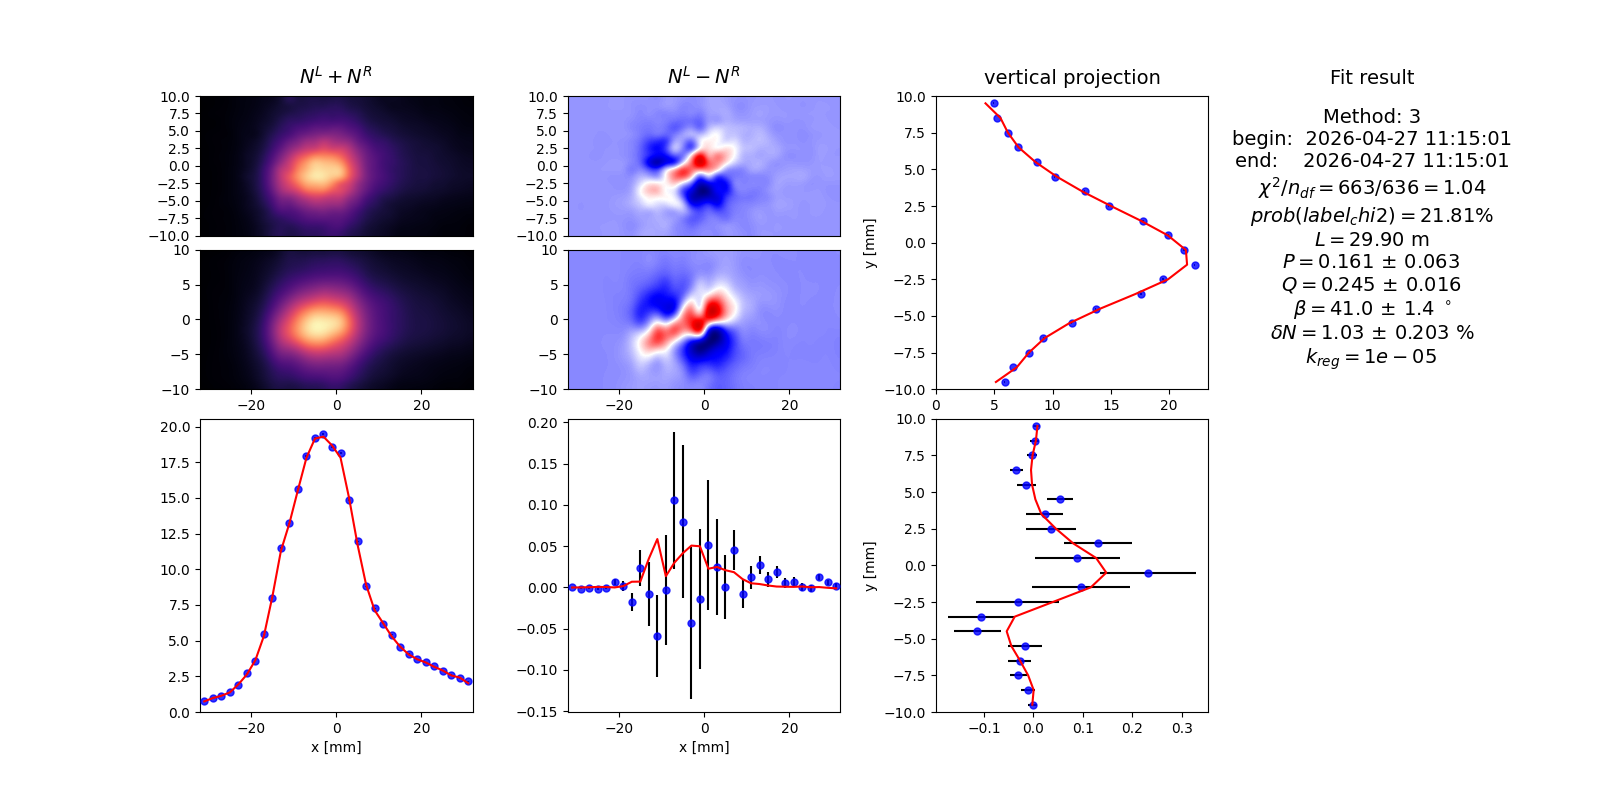
\includegraphics[width=1.\linewidth]{spot_fit_tmp.png}
    \caption{Обработка данных эксперимента}
    \label{fig:placeholder}
\end{figure}
Максимум сдвинут по x на 4 мм, по y на 1,5 мм. Ширина по x -- 21,5 мм; по y -- 9,7 мм.
\subsection{Зависимость от разброса}
$P=1;Q=0,5;\beta=0,7$
\begin{figure}[H]
    \centering
    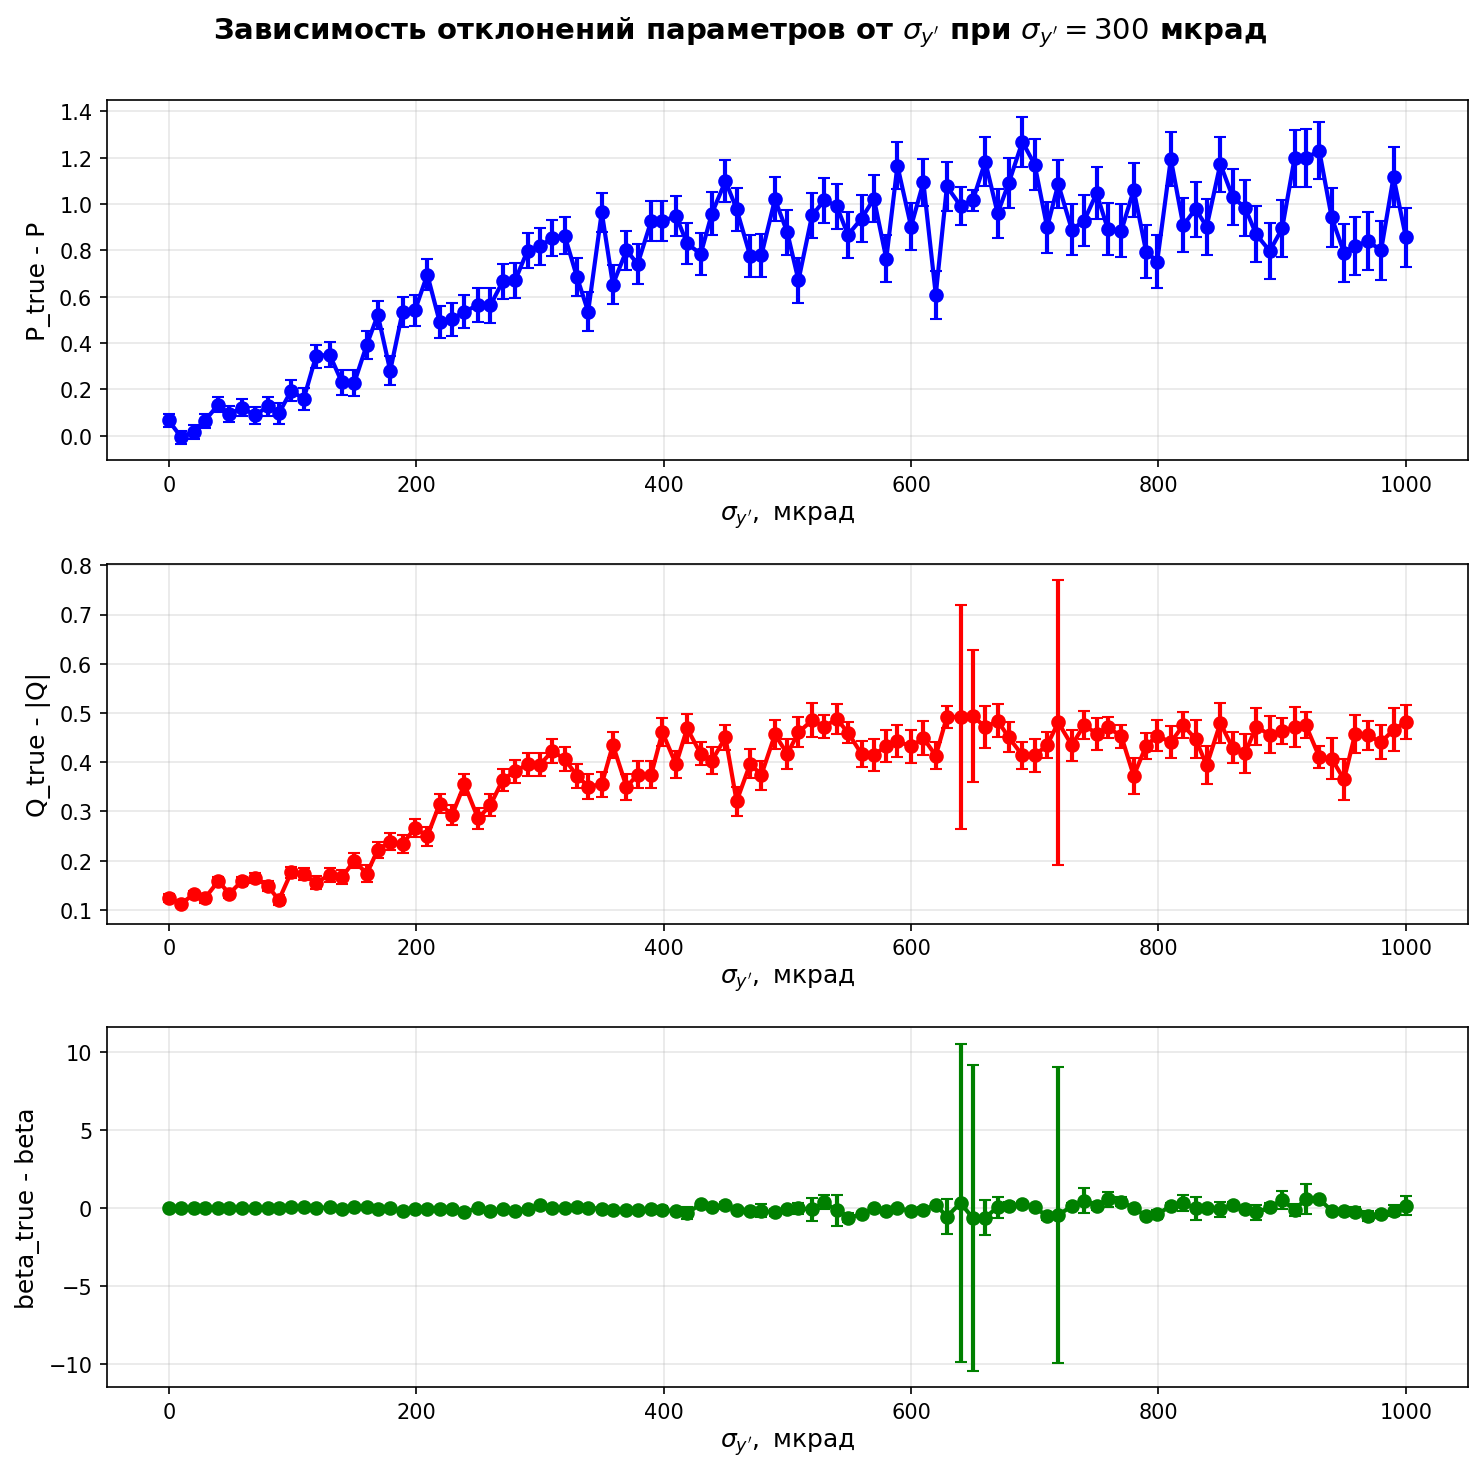
\includegraphics[width=0.7\linewidth]{pictures/подгон_300_y.png}
    \label{fig:placeholder}
\end{figure}

\begin{figure}[H]
    \centering
    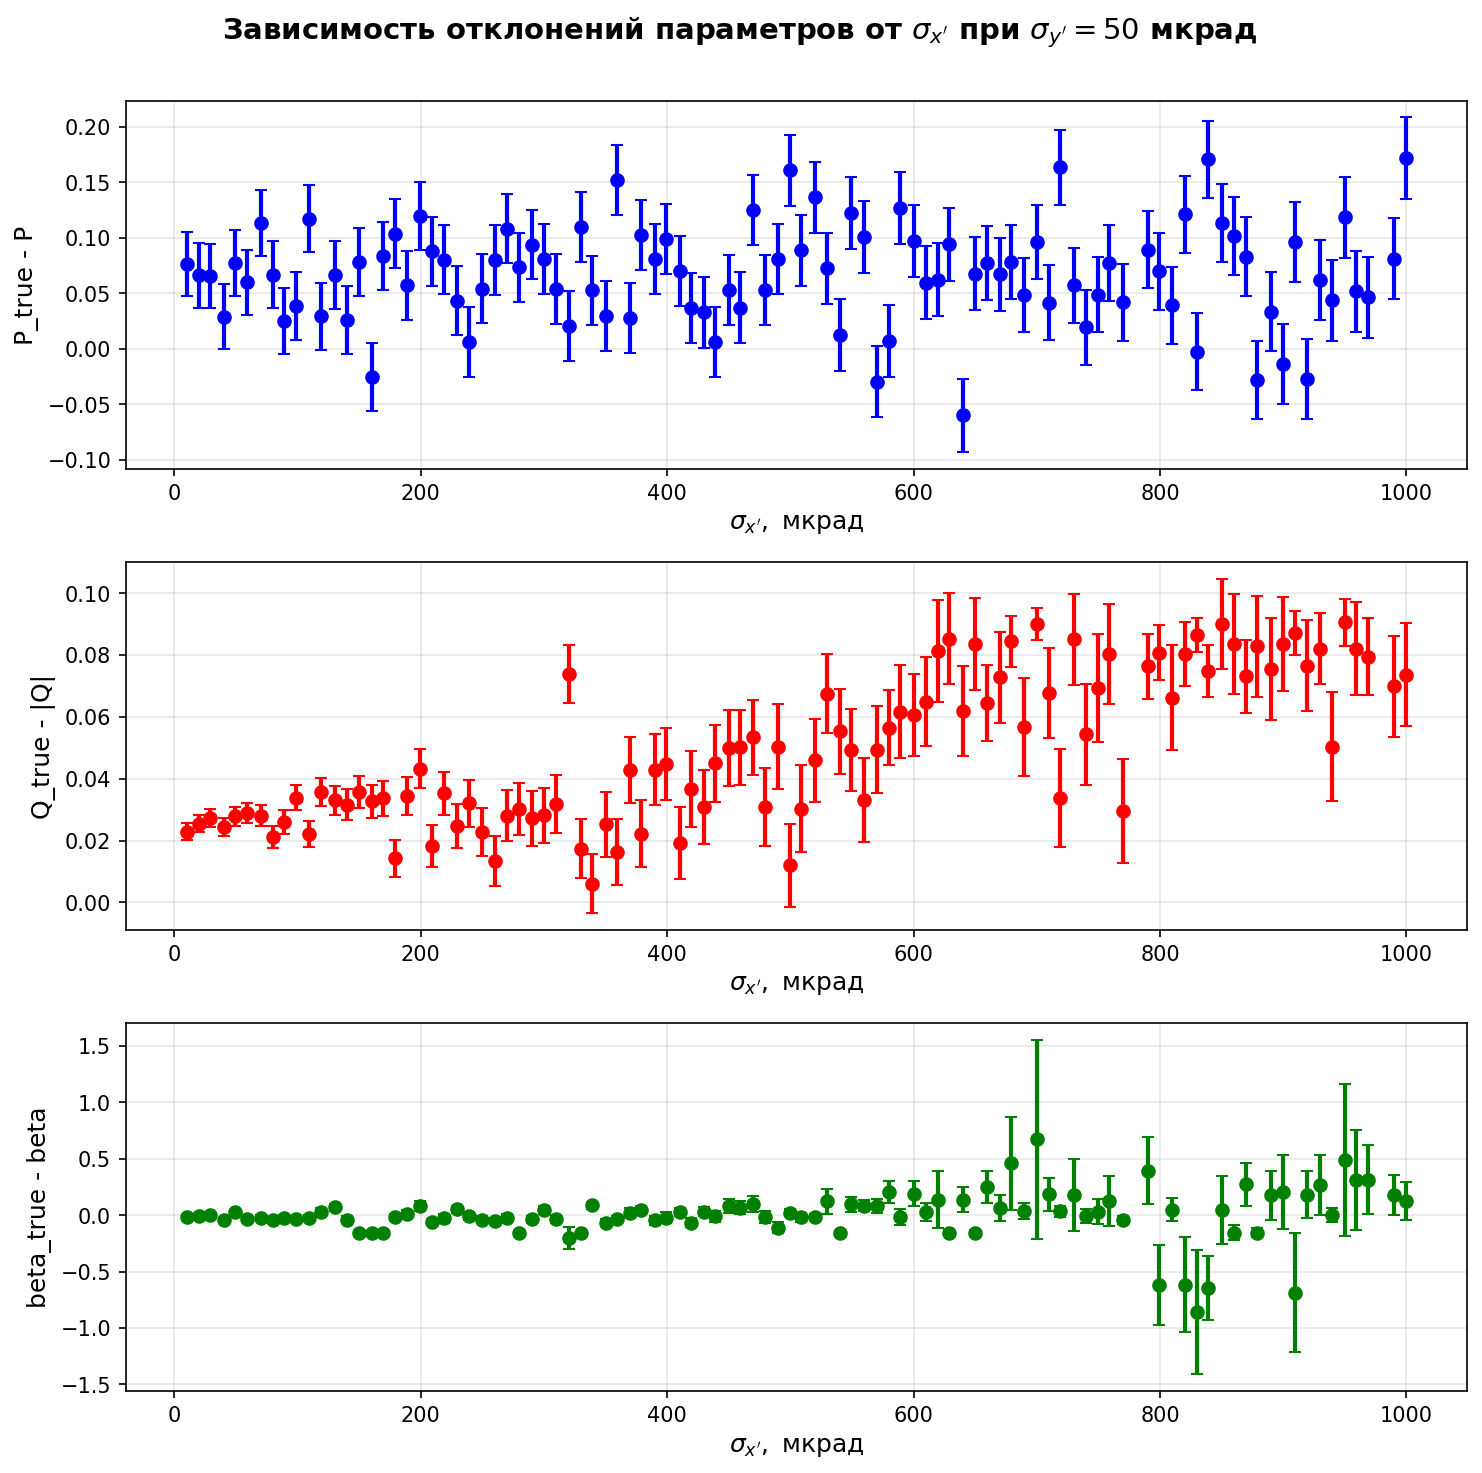
\includegraphics[width=0.7\linewidth]{pictures/подгон_x_50.png}
    \label{fig:placeholder}
\end{figure}
Из графиков видно, что ошибка подгонки поляризации $P$ не зависит от $\sigma_{x'}$, но растёт при увеличении $\sigma_{y'}$. 

\section{Зависимость от параметров}

\section{Подгонка без вещества}

...
\end{document}
